\documentclass[11pt,a4paper]{article}

\usepackage[T1]{fontenc}
\usepackage[utf8]{inputenc}
\usepackage[spanish,es-noquoting,es-tabla]{babel}
\usepackage{amsmath,amssymb,amsthm}
\usepackage{mathtools}
\usepackage{csquotes}
\usepackage{booktabs}
\usepackage{graphicx}
\usepackage{longtable}
\usepackage{caption}
\usepackage{subcaption}
\usepackage{enumitem}
\usepackage[margin=2.4cm]{geometry}
\usepackage{microtype}
\usepackage{xcolor}
% Long dotted identifiers are set on their own line where needed; this only
% relaxes the surrounding prose so it does not overflow the margin.
\setlength{\emergencystretch}{3em}
\usepackage[colorlinks=true,linkcolor=blue!55!black,citecolor=blue!55!black,
            urlcolor=blue!55!black]{hyperref}

\graphicspath{{figs_consolidado/}}

\newcommand{\vect}[1]{\boldsymbol{#1}}
\newcommand{\matr}[1]{\mathbf{#1}}
\newcommand{\erf}{\operatorname{erf}}
\newcommand{\code}[1]{\texttt{#1}}

\theoremstyle{definition}
\newtheorem{finding}{Hallazgo}
\newtheorem{decision}{Decisión}

\title{\textbf{Reporte consolidado del estudio del CRB\\
de la cámara de esquina (NLOS)}\\[3mm]
\large Qué se intentó en las cuatro ramas, qué resultó,\\
y en qué estado queda el repositorio}
\author{Repositorio \code{crb}}
\date{29 de agosto de 2026}

\begin{document}
\maketitle

\begin{abstract}
Este documento consolida en un solo lugar todo el trabajo realizado sobre el
límite de Cramér--Rao (CRB) de la localización de un objeto oculto con una
cámara de esquina NLOS, repartido hasta ahora en cuatro ramas de trabajo con sus
respectivos \emph{pull requests}. El objetivo es que, al retirar esas ramas, no
se pierda ni el razonamiento ni los números: se recogen aquí la cronología, las
decisiones de modelado, los resultados numéricos de cada intento, los hallazgos
de la revisión matemática y de código, y el estado final del repositorio.

El estado final adopta tres decisiones. Primero, el simulador de transientes se
reemplaza por una implementación vectorizada en PyTorch que procesa bloques de
triángulos contra todos los píxeles del SPAD a la vez. Segundo, la grilla de
referencia (\enquote{\emph{baseline}}) pasa de $64\times64$ a $32\times32$ píxeles.
Tercero, el CRB de producción es el de diferencias finitas sobre ese simulador,
con vector de parámetros $\vect\psi=(\rho,\varphi)$ y matriz de información de
Fisher $2\times2$: el simulador nuevo no expone la altura del objeto como
entrada, de modo que $\sigma_h$ deja de estar definida. Con esa configuración,
$\sigma_\rho$ recorre $1.35\,\text{mm}$--$9.0\,\text{cm}$ y $\sigma_\varphi$
recorre $0.75^\circ$--$11.7^\circ$ sobre la rejilla de poses
$\rho\in\{0.5,1.0,1.5\}\,$m, $\varphi\in\{30,60,90,120,150\}^\circ$.
\end{abstract}

\tableofcontents

%=======================================================================
\section{Contexto y objetivo}
\label{sec:contexto}

\subsection{El problema físico}

Una cámara de esquina NLOS ilumina un punto del suelo con un láser pulsado y
observa, con un sensor SPAD que resuelve el tiempo de vuelo, la mancha de luz
que regresa tras rebotar. Si hay un objeto fuera de la línea de vista (detrás de
la esquina), parte de la luz hace un camino de dos rebotes
láser~$\to$~objeto~$\to$~suelo~$\to$~SPAD, y su tiempo de llegada y su
distribución angular contienen información sobre dónde está el objeto.

El simulador del repositorio implementa exactamente ese modelo directo
(\enquote{\emph{forward}}). Para cada triángulo $t$ de la malla de la escena y cada
píxel $p$ del SPAD acumula una contribución
%
\begin{equation}
\label{eq:forward-duro}
I_{t,p}
= I_{\text{láser}}\,\cdot\,\text{área}_t\,\cdot\,
\frac{\cos\theta_1\,\cos\theta_2\,\cos\theta_3\,\cos\theta_4}
     {4\pi^2\, d_1^2\, d_2^2}\,\cdot\,
\underbrace{\mathbf{1}[x_{\text{int}}>0]}_{\text{no oclusión}},
\end{equation}
%
en el \emph{bin} temporal
$j=\lceil (d_1+d_2)/(c\,\Delta t)\rceil$, donde $d_1$ es la distancia
láser--triángulo, $d_2$ la distancia triángulo--píxel, los cuatro cosenos son
productos escalares recortados a cero, y $x_{\text{int}}$ es la abscisa del
corte con el eje de la recta triángulo--píxel, que codifica si la arista de la
esquina oculta ese camino.

\subsection{La pregunta que se quería responder}

La pregunta es de precisión alcanzable, no de reconstrucción: \emph{dada esta
geometría y este sensor, \textquestiondown{}cuál es la mínima varianza que puede tener cualquier
estimador no sesgado de la posición del objeto?} Eso es el CRB. La respuesta se
dibuja como una región de incertidumbre $3\sigma$ en el plano de parámetros
$(\rho,\varphi)$ (coordenadas polares del objeto sobre el suelo), una elipse
---una \enquote{burbuja}--- por cada pose evaluada.

\subsection{Qué se hizo, en una frase}

Se construyeron y compararon dos rutas para calcular ese CRB (la de diferencias
finitas sobre el simulador y la de un \emph{forward} analítico diferenciable),
se llevó la segunda hasta reproducir a la primera dentro de un $10\%$, se
sometió todo a una revisión matemática y de código independiente, y finalmente
se reemplazó el simulador por una versión vectorizada en GPU y se fijó la
grilla de referencia en $32\times32$.

%=======================================================================
\section{Qué es el CRB y cuáles son las dos rutas}
\label{sec:crb}

\subsection{Fisher de Poisson y el CRB}

El SPAD cuenta fotones: el número de cuentas en el \emph{bin} $i$ es una
variable de Poisson de media $g_i(\vect\psi)$, donde
$\vect\psi=(\rho,\varphi)$ (o $(\rho,\varphi,h)$ en las versiones que
estimaban también la altura) y
%
\begin{equation}
g_i(\vect\psi) = y_i(\vect\psi) + b,
\end{equation}
%
con $y_i$ la señal esperada del modelo directo y $b>0$ una tasa de fondo
constante (en todo el estudio $b=0.1$ cuentas/\emph{bin}). Para observaciones
de Poisson independientes, la matriz de información de Fisher es
%
\begin{equation}
\label{eq:fisher}
\matr I(\vect\psi)
= \sum_i \frac{1}{g_i(\vect\psi)}
  \frac{\partial g_i}{\partial\vect\psi}
  \frac{\partial g_i}{\partial\vect\psi}^{\!\top}
= \matr J^\top \operatorname{diag}(1/g)\, \matr J ,
\qquad
\matr J_{im} = \frac{\partial g_i}{\partial\psi_m},
\end{equation}
%
y el CRB es su inversa, $\operatorname{Cov}(\hat{\vect\psi})\succeq
\matr I^{-1}$. De $\matr I^{-1}$ se leen $\sigma_\rho=\sqrt{[\matr
I^{-1}]_{11}}$, $\sigma_\varphi=\sqrt{[\matr I^{-1}]_{22}}$, el error
tangencial $\rho\,\sigma_\varphi$, y la elipse $3\sigma$ se obtiene por
descomposición espectral de $\matr I^{-1}$.

El papel de $b>0$ es doble: es física (hay fondo real) y es matemático, porque
mantiene $g_i$ acotado lejos de cero y por tanto el peso $1/g_i$ finito.

\subsection{El obstáculo: el \emph{forward} no es diferenciable}

Todo el problema del CRB se reduce a obtener el jacobiano $\matr J = \partial
g/\partial\vect\psi$. Pero el \emph{forward} de la
ecuación~\eqref{eq:forward-duro} contiene tres operaciones que destruyen la
diferenciabilidad:
%
\begin{enumerate}[label=(\roman*),leftmargin=*]
  \item el \textbf{binning temporal} $\lceil\cdot\rceil$, constante a trozos:
        mover el objeto un poco no cambia nada hasta que el tiempo de vuelo
        cruza un borde de \emph{bin}, y entonces una masa entera salta de un
        \emph{bin} al siguiente;
  \item la \textbf{máscara de oclusión} $\mathbf 1[x_{\text{int}}>0]$, un
        escalón de Heaviside;
  \item los \textbf{recortes} $\max(0,\cdot)$ de los cuatro cosenos, con un
        codo no diferenciable en el origen.
\end{enumerate}

De ahí las dos rutas.

\subsection{Ruta FD: diferenciar numéricamente el simulador}

Se toma el simulador tal cual (con sus escalones) y se aproxima cada columna
del jacobiano por una diferencia central,
%
\begin{equation}
\matr J_{:,m} \approx \frac{g(\vect\psi+\delta_m \vect e_m) -
                            g(\vect\psi-\delta_m \vect e_m)}{2\delta_m},
\end{equation}
%
con pasos $\delta_\rho = 0.01\,$m y $\delta_\varphi = 0.5^\circ$. Es la ruta de
producción: vive en \code{crb\_polar\_functions.py} y usa el modelo de malla
completo, sin aproximaciones de modelado. Su debilidad es numérica: sobre un
\emph{forward} escalonado la diferencia finita mezcla mesetas (derivada cero)
con saltos de \emph{bin} (derivada $\propto 1/\delta$), y el resultado depende
del paso $\delta$. Lo que la rescata en la práctica es la densificación de la
malla: con miles de triángulos las distancias por triángulo se reparten y el
jacobiano agregado se auto-promedia.

\subsection{Ruta analítica: suavizar y derivar exacto}

Se reemplazan las tres operaciones no diferenciables por versiones $C^\infty$
con un parámetro de anchura, se construye el \emph{forward} suave en
\code{sympy}, y se deriva de forma \emph{exacta} y simbólica:
%
\begin{center}
\begin{tabular}{@{}lll@{}}
\toprule
Operación dura & Reemplazo suave & Anchura \\
\midrule
$\lceil\cdot\rceil$ (masa en un \emph{bin}) &
  diferencia de $\erf$ &
  $\tau$ \\
$\mathbf 1[x_{\text{int}}>0]$ (oclusión) &
  sigmoide $\sigma(\kappa\, x_{\text{int}})$ &
  $1/\kappa$ \\
$\max(0,x)$ (recortes) &
  \emph{softplus} $\log(1+e^{\beta x})/\beta$ &
  $1/\beta$ \\
\bottomrule
\end{tabular}
\end{center}

La justificación del primer reemplazo es la que da nombre a la construcción: en
lugar de asignar toda la masa del triángulo al \emph{bin} que contiene su
tiempo de vuelo $t_0$, se reparte con un núcleo gaussiano de anchura $\tau$ y
se integra sobre el \emph{bin} $[j\Delta t,(j{+}1)\Delta t)$, lo que da
%
\begin{equation}
\label{eq:erf}
S_{ij}(t_0) = \tfrac12\left[
  \erf\!\left(\frac{(j{+}1)\Delta t - t_0}{\sqrt2\,\tau}\right)
- \erf\!\left(\frac{j\Delta t - t_0}{\sqrt2\,\tau}\right)\right],
\end{equation}
%
que es real-analítica en $t_0$, suma exactamente $1$ sobre todos los
\emph{bins} (conserva la masa) y converge al \emph{binning} duro cuando
$\tau\to0$. Las figuras~\ref{fig:smoothing} muestran los tres reemplazos.

\begin{figure}[htbp]
\centering
\begin{subfigure}{0.48\textwidth}
  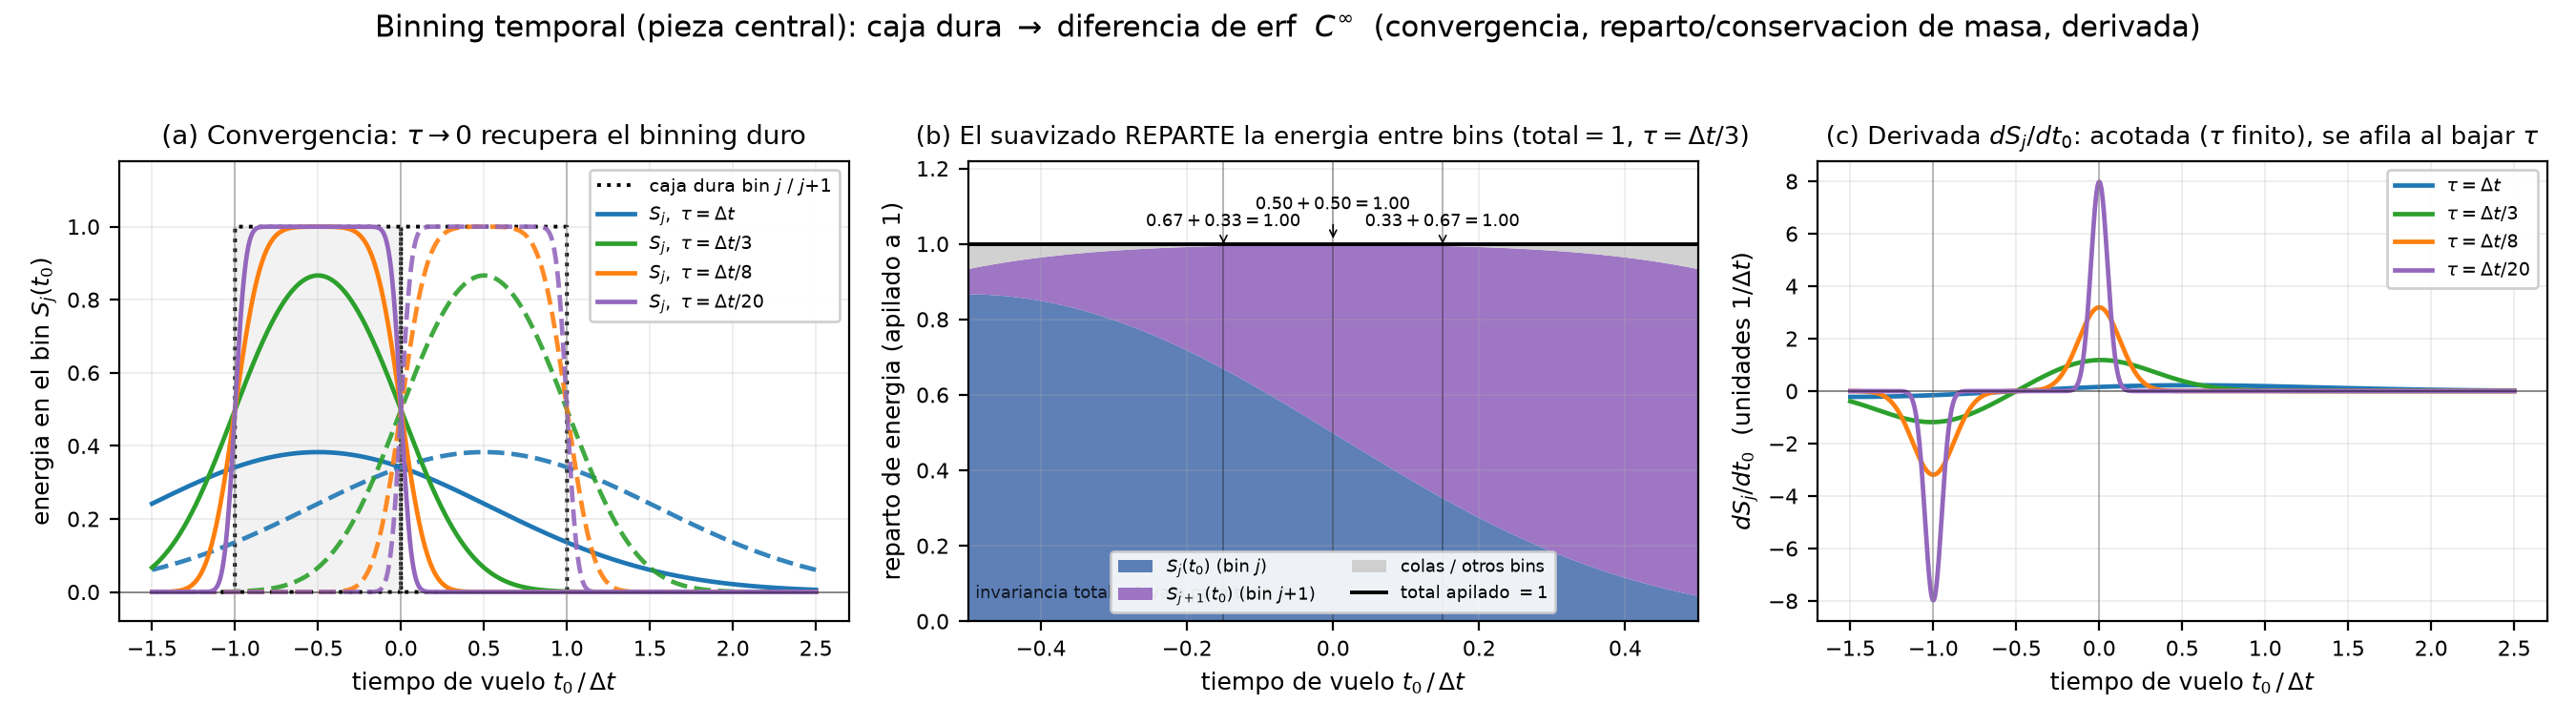
\includegraphics[width=\linewidth]{smoothing_binning.png}
  \caption{\emph{Binning} temporal: $\lceil\cdot\rceil \to \erf$
           (ecuación~\eqref{eq:erf}).}
\end{subfigure}\hfill
\begin{subfigure}{0.48\textwidth}
  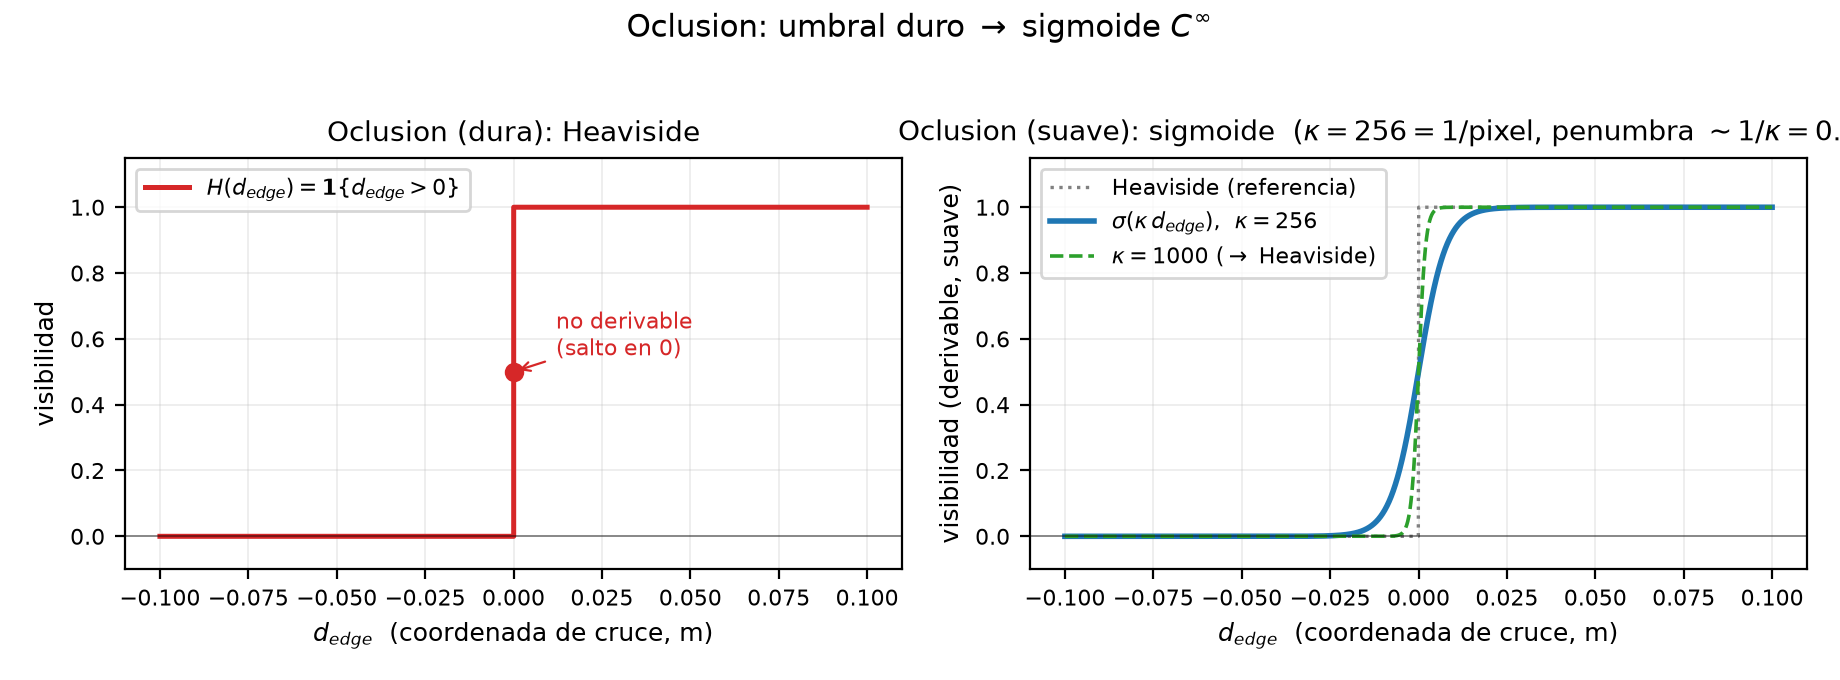
\includegraphics[width=\linewidth]{smoothing_occlusion.png}
  \caption{Oclusión: escalón $\to$ sigmoide de penumbra.}
\end{subfigure}

\vspace{3mm}
\begin{subfigure}{0.48\textwidth}
  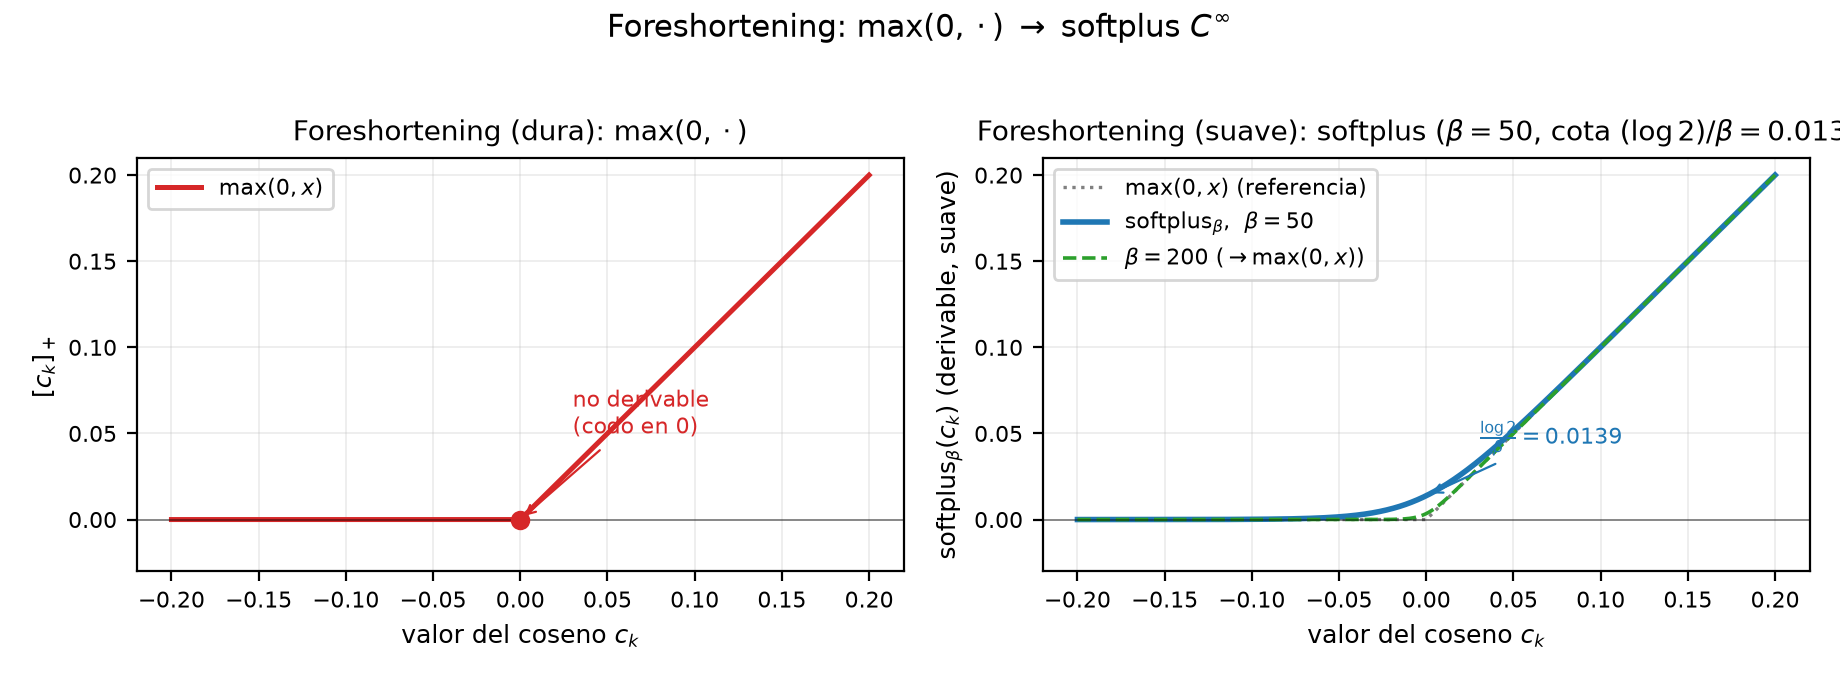
\includegraphics[width=\linewidth]{smoothing_foreshortening.png}
  \caption{Recorte de los cosenos: $\max(0,\cdot) \to$ \emph{softplus}.}
\end{subfigure}
\caption{Los tres reemplazos que convierten el \emph{forward} del simulador en
una función $C^\infty$ derivable en forma cerrada. Figuras heredadas de la rama
de suma sobre malla, con la configuración final
$\kappa=256$, $\tau=\Delta t/\sqrt{12}$.}
\label{fig:smoothing}
\end{figure}

Sobre esa base, el documento \code{analytic\_forward\_crb.tex} desarrollaba una
justificación matemática completa: los bloques \enquote{suaves} del simulador
(distancias, tiempos de vuelo, cosenos) ya son $C^\infty$ fuera de
degeneraciones (lema de la norma euclídea); el diagnóstico de la no
diferenciabilidad se hace con el \textbf{teorema de la función implícita} para
identificar la superficie de salto y con el \textbf{teorema de Rademacher} para
situar el conjunto de no diferenciabilidad; las herramientas para el paso al
límite son la \textbf{convergencia dominada}, la \textbf{derivación bajo la
integral} (Leibniz) y las \textbf{aproximaciones de la identidad}
(\emph{mollifiers}); y el cierre es que el CRB es $C^\infty$ donde $\matr
I\succ0$. Un resultado negativo importante de ese desarrollo es la
\textbf{inconsistencia de la diferencia finita en un salto}: en el límite duro
la derivada diverge y la Fisher \enquote{dura} no existe en sentido clásico, lo cual es
precisamente la razón de suavizar en lugar de intentar derivar el modelo duro.

%=======================================================================
\section{Cronología: qué se intentó en cada rama}
\label{sec:cronologia}

Las cuatro ramas son incrementales: cada una añade un ingrediente a la
anterior y se mide contra la misma referencia FD.

\begin{center}
\small
\begin{tabular}{@{}lp{4.3cm}p{5.1cm}p{3.9cm}@{}}
\toprule
PR & Rama & Aporte & Resultado en una línea \\
\midrule
\#1 & \code{regenerate-} \code{crb-ellipse-plots} &
  regenera los PNG de la ruta FD como burbujas en $(\rho,\varphi)$ &
  solo figuras; no toca código \\
\addlinespace
\#2 & \code{analytic-} \code{differentiable-forward} &
  \emph{forward} analítico suave, base cualitativa &
  comparable solo en \emph{forma} \\
\addlinespace
\#3 & \code{analytic-forward-} \code{physical-grid} &
  (a) amplitud física + (b) rejilla del simulador &
  $\sigma_\rho^{\text{an}}/\sigma_\rho^{\text{FD}}\in[0.50,0.85]$;
  sesgo de cuadratura puntual $\sim1.5\times$ \\
\addlinespace
\#4 & \code{analytic-forward-} \code{mesh-sum} &
  (a)+(b)+(c) suma sobre la malla real densificada &
  razón $\sigma_\rho\in[1.08,1.10]$;
  razón $\sigma_\varphi\in[1.06,1.12]$ \\
\bottomrule
\end{tabular}
\end{center}

%-----------------------------------------------------------------------
\subsection{PR\#1 --- Regeneración de las regiones CRB por la ruta FD}
\label{sec:pr1}

\paragraph{Qué se hizo.}
Se regeneraron las figuras del CRB calculado por diferencias finitas para que
se dibujaran como \emph{elipses en el plano de parámetros} $(\rho,\varphi)$
---burbujas centradas en cada pose--- en lugar del empuje hacia adelante
(\enquote{\emph{pushforward}}) al plano físico $xy$, que producía formas de gota
difíciles de leer. En el código esto corresponde a llamar
\code{plot\_crb\_regions\_polar(..., use\_physical\_region=False)}, con
\code{rlim=2.0}, etiquetas radiales a dos decimales y fuentes reducidas.

El cálculo se hacía con el \emph{script}
\code{regenerate\_crb\_standard\_regions.py}, que cargaba las celdas
$1,3,5,7,8$ del \emph{notebook} \code{simulation\_polar\_clean.ipynb} para
obtener la función \code{simulation} y sus parámetros, y luego llamaba a
\code{compute\_crb\_grid\_polar} dos veces: una con
$\vect\psi=(\rho,\varphi)$ (Fisher $2\times2$) y otra con
$\vect\psi=(\rho,\varphi,h)$ (Fisher $3\times3$).

\paragraph{Qué se aprendió.}
El diff de esta rama frente a \code{main} era exactamente cuatro PNG: los que
el script escribe. La revisión confirmó que la representación en el plano de
parámetros es la correcta para leer $\sigma_\rho$ y $\sigma_\varphi$
directamente de los semiejes. El código del CRB por FD ya vivía en
\code{main} (\code{crb\_polar\_functions.py}); PR\#1 no lo modificaba.

\begin{figure}[htbp]
\centering
\begin{subfigure}{0.48\textwidth}
  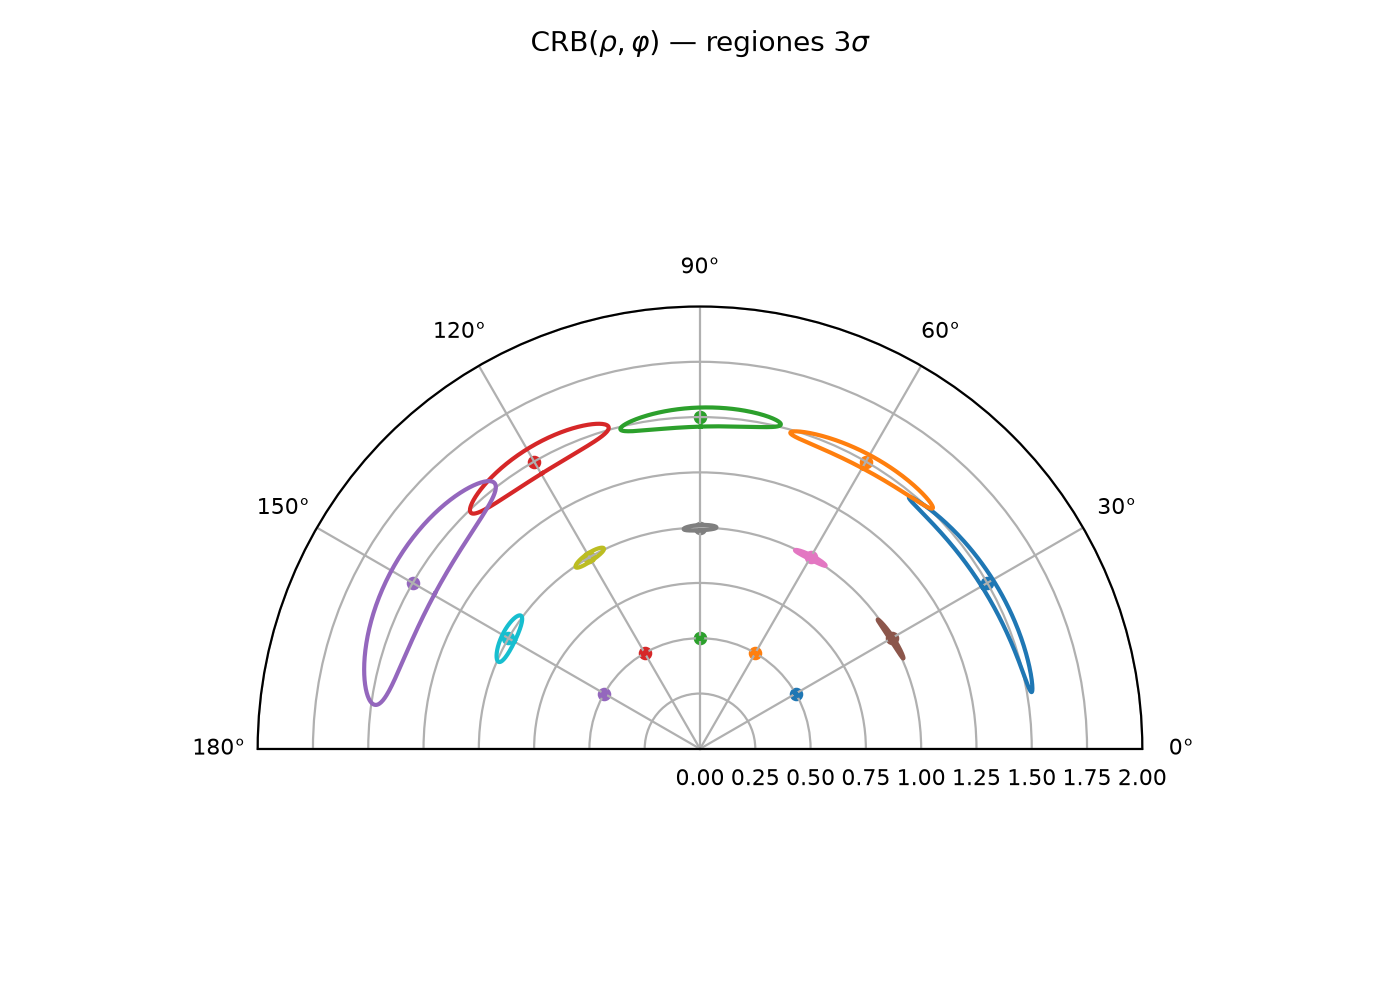
\includegraphics[width=\linewidth]{pr1_fd_fixed_h.png}
  \caption{CRB$(\rho,\varphi)$, Fisher $2\times2$.}
\end{subfigure}\hfill
\begin{subfigure}{0.48\textwidth}
  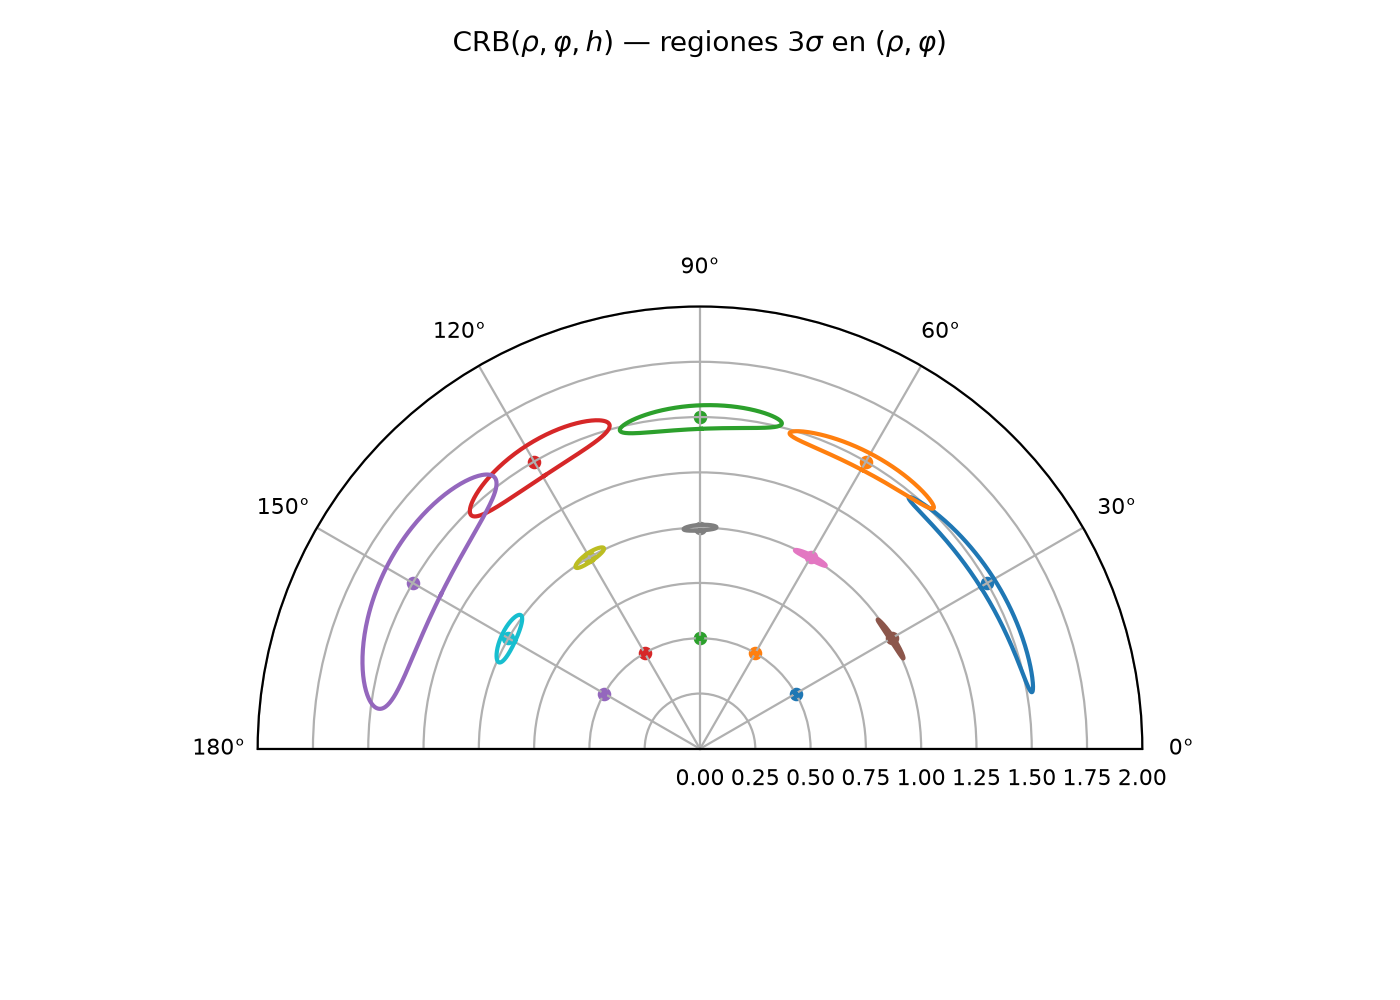
\includegraphics[width=\linewidth]{pr1_fd_with_h.png}
  \caption{CRB$(\rho,\varphi,h)$, Fisher $3\times3$, proyectado en
           $(\rho,\varphi)$.}
\end{subfigure}
\caption{PR\#1: regiones $3\sigma$ de la ruta FD sobre el simulador antiguo
($64\times64$, \code{subpixel\_dim=4}). Estimar además la altura $h$ ensancha
las burbujas, porque la información se reparte entre tres parámetros.}
\label{fig:pr1}
\end{figure}

%-----------------------------------------------------------------------
\subsection{PR\#2 --- \emph{Forward} analítico diferenciable (base cualitativa)}
\label{sec:pr2}

\paragraph{Qué se hizo.}
Se construyó por primera vez el \emph{forward} suave completo en \code{sympy},
con los tres reemplazos de la sección~\ref{sec:crb}, y su jacobiano exacto. El
módulo es \code{crb\_analytic\_forward.py} y el documento que lo justifica es
\code{docs/analytic\_forward\_crb.tex}, con el desarrollo paso a paso
(construcción, derivada, justificación matemática con teoremas, Fisher de
Poisson, validación y resultados).

Esta rama es deliberadamente una \textbf{base cualitativa}. Su configuración no
pretende ser fiel al simulador:
%
\begin{itemize}[leftmargin=*]
  \item la faceta se modela como un \textbf{punto} colocado en $z=h$ (no en el
        centroide de la malla, que está en $\approx h/2$);
  \item la amplitud se pliega en una \textbf{ganancia libre} $G=10^5$ constante,
        de modo que $\partial y/\partial h$ representa \enquote{subir una faceta de
        tamaño fijo}, no el área $\propto h$ del simulador;
  \item usa su \textbf{propia rejilla} $8\times8$ con FOV $0.5$ y centro
        $-0.25$, en lugar de la $64\times64$ / FOV $0.25$ / centro $-0.125$ del
        simulador;
  \item las anchuras de suavizado son genéricas: $\kappa=60$, $\tau=\Delta t$.
\end{itemize}

\paragraph{Qué se aprendió.}
La validación intrínseca funcionó a la primera y con margen: el jacobiano
simbólico coincide con una diferencia central del \emph{mismo} \emph{forward}
suave con error máximo $5.0\cdot10^{-10}$. Es decir, la derivada exacta está
bien implementada. Pero las magnitudes absolutas del CRB \textbf{no son
comparables} con la ruta FD, porque los modelos son distintos y $G$ es
arbitraria: la comparación honesta es de \emph{forma}, tras normalizar la
escala. Con esa normalización, la relación de aspecto media resultó $4.96$
frente a $8.22$ del FD, y la inclinación de las elipses fue consistente.

La conclusión operativa de PR\#2 fue: la derivada exacta es claramente mejor
condicionada que la FD (que sufre el ruido de discretización de los escalones),
pero para que el CRB analítico signifique algo hay que ponerlo en las unidades
y la geometría del simulador. Eso motivó PR\#3 y PR\#4.

\begin{table}[htbp]
\centering
\caption{PR\#2: CRB analítico (A) frente a FD (F) sobre la rejilla estándar.
Las columnas $\sigma$ analíticas \emph{no} son comparables en magnitud con las
FD (ganancia $G$ libre, geometría y rejilla propias); lo comparable es
\code{asp} (eje mayor/eje menor) y la inclinación.}
\label{tab:pr2}
\small
\begin{tabular}{@{}rr rrr rrr@{}}
\toprule
& & \multicolumn{3}{c}{Analítico (base cualitativa)}
  & \multicolumn{3}{c}{FD (referencia)} \\
\cmidrule(lr){3-5}\cmidrule(lr){6-8}
$\rho$ [m] & $\varphi$ [$^\circ$]
& $\sigma_\rho$ [m] & $\sigma_\varphi$ [$^\circ$] & asp
& $\sigma_\rho$ [m] & $\sigma_\varphi$ [$^\circ$] & asp \\
\midrule
0.50 & 30  & 0.001306 & 0.4259 & 6.85  & 0.0006859 & 0.5091 & 19.21 \\
0.50 & 60  & 0.001184 & 0.2891 & 4.50  & 0.0006779 & 0.4401 & 14.03 \\
0.50 & 90  & 0.001390 & 0.2838 & 3.64  & 0.0007805 & 0.3846 & 9.61  \\
0.50 & 120 & 0.002027 & 0.2448 & 2.13  & 0.001116  & 0.4116 & 7.08  \\
0.50 & 150 & 0.003547 & 0.3478 & 1.72  & 0.001847  & 0.5484 & 5.70  \\
1.00 & 30  & 0.001382 & 0.5349 & 9.84  & 0.003406  & 2.012  & 13.06 \\
1.00 & 60  & 0.001201 & 0.3740 & 6.17  & 0.003448  & 1.478  & 8.23  \\
1.00 & 90  & 0.001400 & 0.3807 & 5.01  & 0.004197  & 1.416  & 6.19  \\
1.00 & 120 & 0.001992 & 0.3231 & 2.88  & 0.006299  & 1.460  & 4.20  \\
1.00 & 150 & 0.003395 & 0.4680 & 2.43  & 0.01086   & 2.214  & 3.70  \\
1.50 & 30  & 0.002255 & 0.8964 & 10.86 & 0.01207   & 6.763  & 12.10 \\
1.50 & 60  & 0.001918 & 0.6378 & 6.76  & 0.01215   & 4.687  & 7.23  \\
1.50 & 90  & 0.002228 & 0.6684 & 5.59  & 0.01486   & 4.664  & 5.66  \\
1.50 & 120 & 0.003150 & 0.5646 & 3.19  & 0.02185   & 4.717  & 3.84  \\
1.50 & 150 & 0.005356 & 0.8426 & 2.77  & 0.03747   & 7.432  & 3.51  \\
\midrule
\multicolumn{2}{@{}l}{Aspecto medio}
& \multicolumn{3}{c}{$4.96$} & \multicolumn{3}{c}{$8.22$} \\
\bottomrule
\end{tabular}
\end{table}

\begin{figure}[htbp]
\centering
\begin{subfigure}{0.48\textwidth}
  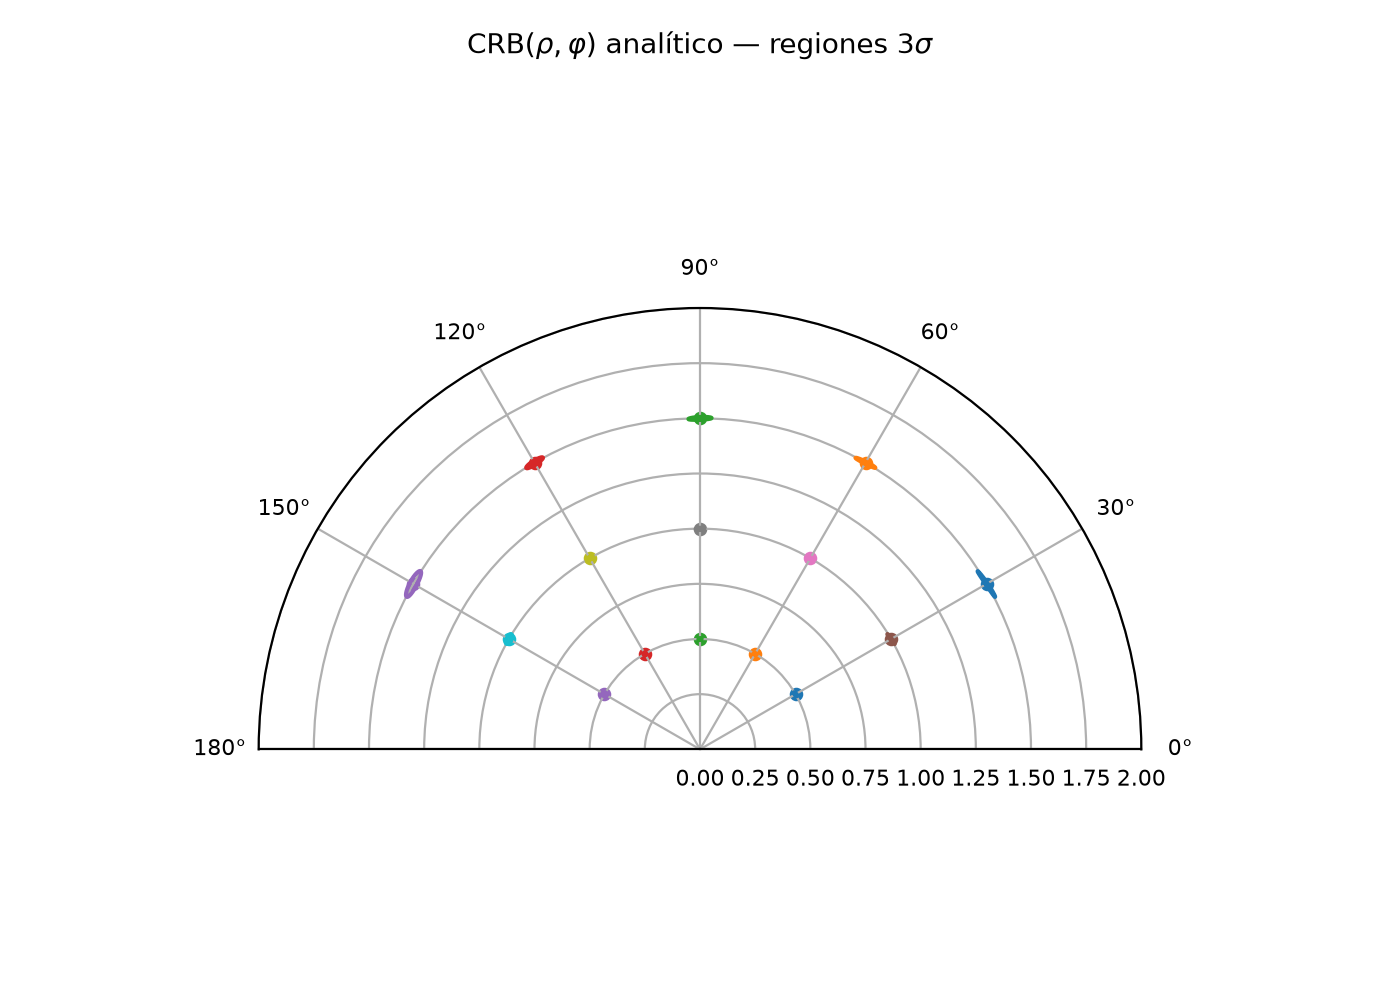
\includegraphics[width=\linewidth]{pr2_analytic_fixed_h.png}
  \caption{Burbujas del CRB analítico base, escala propia.}
\end{subfigure}\hfill
\begin{subfigure}{0.48\textwidth}
  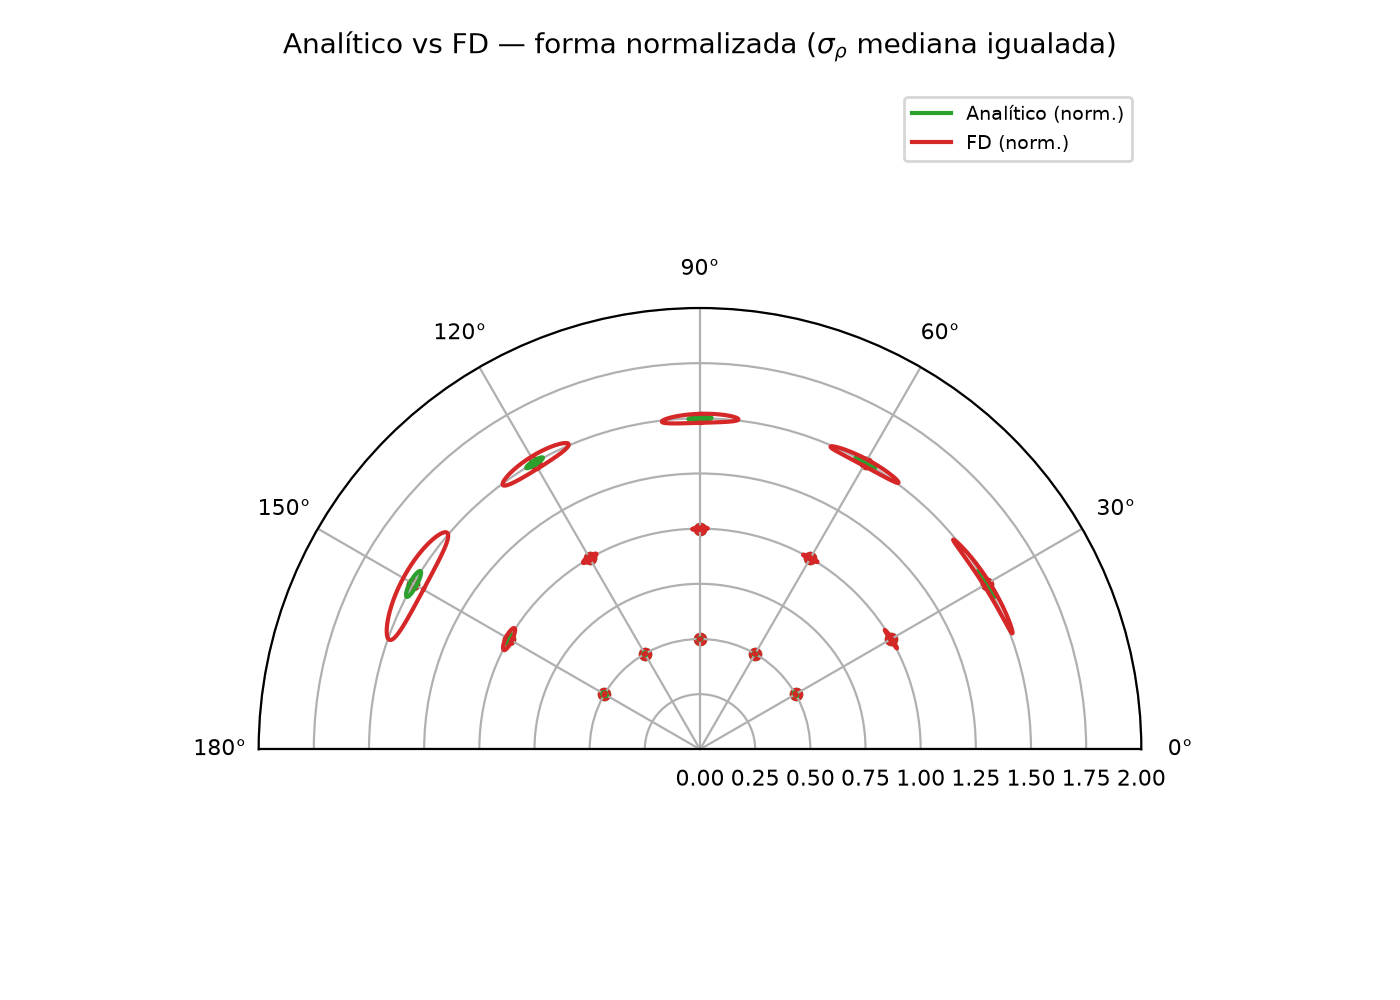
\includegraphics[width=\linewidth]{pr2_shapenorm.png}
  \caption{Superposición normalizada en forma: analítico (verde) vs FD (rojo).}
\end{subfigure}
\caption{PR\#2: al no ser comparables las magnitudes, la superposición se hace
escalando ambas familias de elipses al mismo $\sigma_\rho$ mediano. El escalado
es isótropo alrededor del centro, así que preserva aspecto e inclinación.}
\label{fig:pr2}
\end{figure}

%-----------------------------------------------------------------------
\subsection{PR\#3 --- Amplitud física y rejilla del simulador (a)+(b)}
\label{sec:pr3}

\paragraph{Qué se hizo.}
Dos correcciones sobre PR\#2:
%
\begin{description}[leftmargin=*,style=nextline]
  \item[(a) Amplitud física.] Se elimina la ganancia libre $G=10^5$ y se pone
        la amplitud real del simulador: $I_{\text{láser}}=1000$ y área efectiva
        $\text{área}_{\text{eff}}=w\cdot h$ con $w=0.5\,$m fijo y $h$ la altura
        estimada, de modo que la magnitud escala con $h$ igual que en la malla.
        No queda ningún parámetro de ganancia libre.
  \item[(b) Rejilla del simulador.] Se adopta la rejilla real: $64\times64$
        píxeles, FOV $0.25$, centro $-0.125$, y el tamaño de \emph{bin}
        verdadero $\Delta t = 3.9\cdot10^{-10}\,$s. El centroide de la faceta se
        coloca en $z=h/2$, como en la malla.
\end{description}

\paragraph{Qué se aprendió: el hallazgo central de esta rama.}
La corrección funcionó para lo que buscaba ---$\sigma_\rho$ y $\sigma_\varphi$
analíticos quedaron en las \emph{mismas unidades} que los FD, y del mismo
orden--- pero reveló un problema de modelado más profundo:

\begin{finding}[Sesgo sistemático de cuadratura puntual]
\label{find:cuadratura}
Evaluar la radiometría en \textbf{un solo punto} (el centroide, con área
$w\cdot h$) es una regla del punto medio para una integral de superficie, y
\textbf{sobreestima la intensidad en un factor $\approx1.5$} frente a la suma
sobre la malla. Medido en $\vect\psi=(1\,\text{m},75^\circ,1\,\text{m})$: la
energía total puntual da $2617$ frente a $1749$ de la suma sobre $512$
triángulos, una razón de $1.50$, con un error $L_1$ por píxel de $\approx50\%$.
La causa dominante es la \textbf{oclusión}: el centroide está visible para casi
todos los píxeles mientras que parte de la faceta real de $0.5\times1\,$m está
ocluida. A eso se añade la no linealidad de $1/d_2^2$ y de los cosenos sobre
una faceta extendida a distancias de $\sim1\,$m.
\end{finding}

Como consecuencia, $\sigma_\varphi^{\text{an}}/\sigma_\varphi^{\text{FD}}$ baja
hasta $\approx0.57$ y el rango global de
$\sigma_\rho^{\text{an}}/\sigma_\rho^{\text{FD}}$ queda en $[0.50,0.85]$.

\begin{finding}[Endurecer el suavizado \emph{no} corrige el sesgo]
\label{find:no-converge}
Una afirmación inicial de esta rama era que al llevar $\tau\to0$,
$1/\kappa,1/\beta\to0$ el CRB analítico \enquote{converge hacia el FD}. Es
\textbf{falso}. Al endurecer, esta variante converge a su \emph{propio}
\emph{forward} duro \emph{de faceta puntual} (verificado: el error $L_1$ por
píxel baja de $15.9\%$ a $0.34\%$ respecto a ese duro puntual), \textbf{no} al
\emph{forward} de malla del simulador. El error de cuadratura es sistemático y
sobrevive a cualquier endurecimiento. La única corrección es sumar sobre la
malla, que es exactamente lo que hace PR\#4.
\end{finding}

Un efecto secundario, más pequeño, es que las anchuras de suavizado seguían
siendo genéricas: $\tau=\Delta t$ y $\kappa=60$ dan una penumbra de $1/\kappa =
1.67\,$cm, que son $\approx4.3$ píxeles del simulador (\emph{pitch}
$0.25/64=0.39\,$cm). Es decir, más gruesas que la discretización que pretenden
imitar, y parte del desajuste de forma (aspecto medio $9.36$ frente a $8.22$
del FD) viene de ahí.

\begin{table}[htbp]
\centering
\caption{PR\#3 (a)+(b): ahora las columnas $\sigma$ \emph{sí} están en las
mismas unidades que las FD. La razón analítico/FD queda sistemáticamente por
debajo de $1$ ($[0.50,0.85]$ en $\sigma_\rho$), que es la huella del sesgo de
cuadratura puntual del hallazgo~\ref{find:cuadratura}.}
\label{tab:pr3}
\small
\begin{tabular}{@{}rr rrr rrr r@{}}
\toprule
& & \multicolumn{3}{c}{Analítico (a)+(b)} & \multicolumn{3}{c}{FD (referencia)}
& \\
\cmidrule(lr){3-5}\cmidrule(lr){6-8}
$\rho$ [m] & $\varphi$ [$^\circ$]
& $\sigma_\rho$ [m] & $\sigma_\varphi$ [$^\circ$] & asp
& $\sigma_\rho$ [m] & $\sigma_\varphi$ [$^\circ$] & asp
& razón $\sigma_\rho$ \\
\midrule
0.50 & 30  & 0.0005795 & 0.3799 & 15.26 & 0.0006859 & 0.5091 & 19.21 & 0.845 \\
0.50 & 60  & 0.0005580 & 0.2838 & 10.13 & 0.0006779 & 0.4401 & 14.03 & 0.823 \\
0.50 & 90  & 0.0006579 & 0.2717 & 7.75  & 0.0007805 & 0.3846 & 9.61  & 0.843 \\
0.50 & 120 & 0.0009266 & 0.2364 & 4.65  & 0.001116  & 0.4116 & 7.08  & 0.830 \\
0.50 & 150 & 0.001541  & 0.3056 & 3.58  & 0.001847  & 0.5484 & 5.70  & 0.834 \\
1.00 & 30  & 0.002008  & 1.407  & 17.83 & 0.003406  & 2.012  & 13.06 & 0.589 \\
1.00 & 60  & 0.001912  & 1.078  & 11.57 & 0.003448  & 1.478  & 8.23  & 0.555 \\
1.00 & 90  & 0.002288  & 1.115  & 9.25  & 0.004197  & 1.416  & 6.19  & 0.545 \\
1.00 & 120 & 0.003268  & 0.9953 & 5.52  & 0.006299  & 1.460  & 4.20  & 0.519 \\
1.00 & 150 & 0.005424  & 1.379  & 4.56  & 0.01086   & 2.214  & 3.70  & 0.499 \\
1.50 & 30  & 0.008991  & 6.318  & 18.20 & 0.01207   & 6.763  & 12.10 & 0.745 \\
1.50 & 60  & 0.008545  & 4.875  & 11.74 & 0.01215   & 4.687  & 7.23  & 0.703 \\
1.50 & 90  & 0.01034   & 5.253  & 9.64  & 0.01486   & 4.664  & 5.66  & 0.696 \\
1.50 & 120 & 0.01500   & 4.821  & 5.79  & 0.02185   & 4.717  & 3.84  & 0.687 \\
1.50 & 150 & 0.02504   & 6.950  & 4.94  & 0.03747   & 7.432  & 3.51  & 0.668 \\
\midrule
\multicolumn{2}{@{}l}{Aspecto medio}
& \multicolumn{3}{c}{$9.36$} & \multicolumn{3}{c}{$8.22$} & \\
\bottomrule
\end{tabular}
\end{table}

\begin{figure}[htbp]
\centering
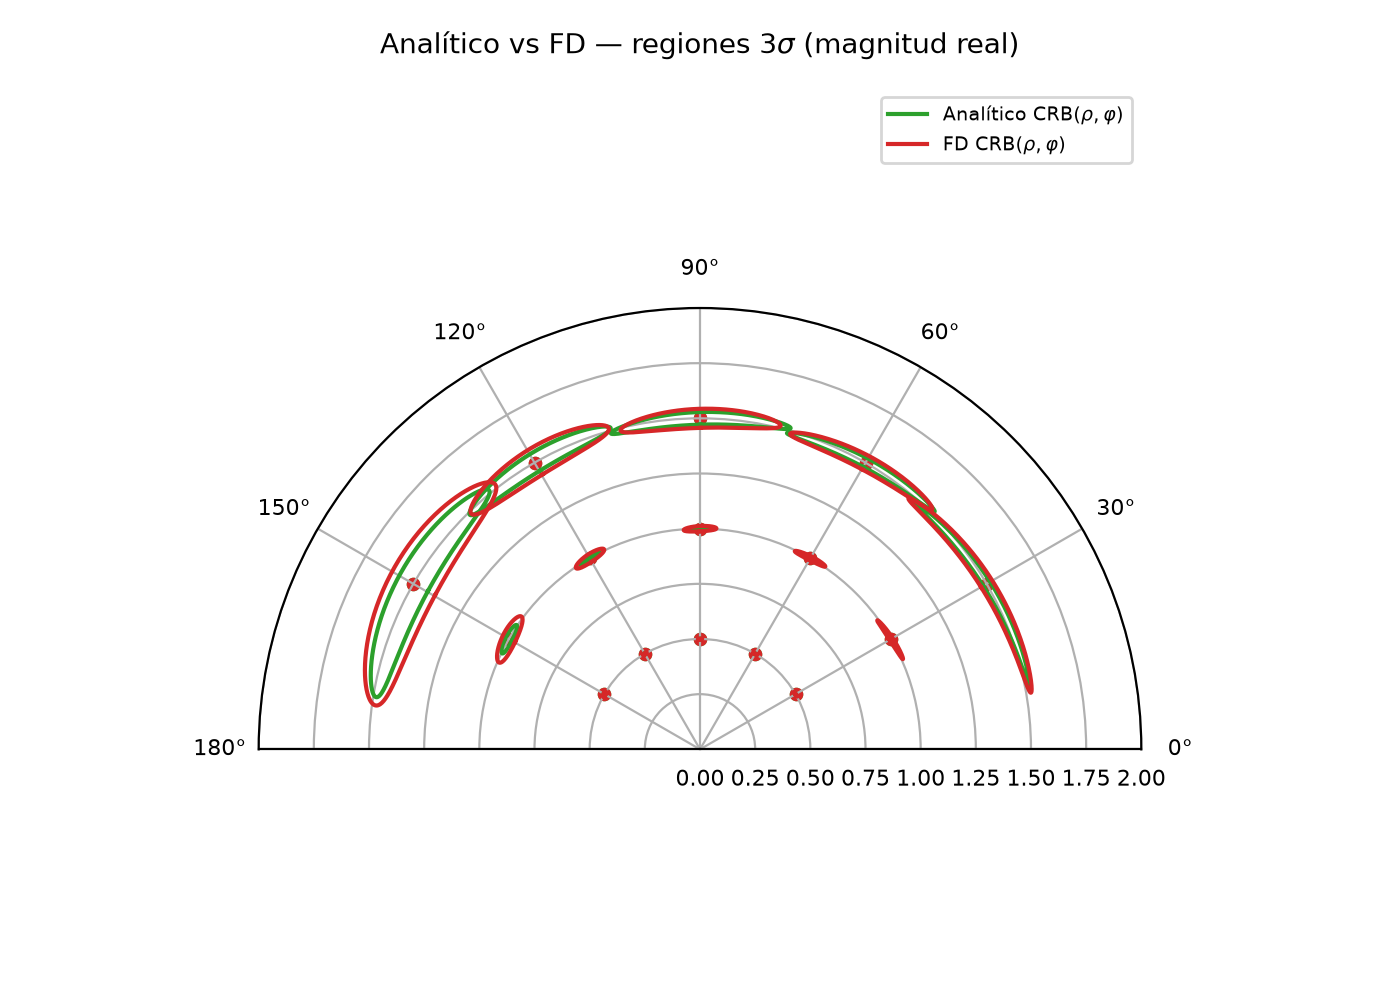
\includegraphics[width=0.62\textwidth]{pr3_overlay.png}
\caption{PR\#3: superposición a magnitud real (sin normalizar) del CRB
analítico (a)+(b) sobre el FD. Las escalas ya coinciden, pero las elipses
analíticas son sistemáticamente más pequeñas: el modelo puntual \enquote{ve} más señal
de la que hay y por tanto promete más precisión de la real.}
\label{fig:pr3}
\end{figure}

%-----------------------------------------------------------------------
\subsection{PR\#4 --- Suma sobre la malla real densificada (a)+(b)+(c)}
\label{sec:pr4}

\paragraph{Qué se hizo.}
Se añadió el ingrediente que faltaba:
%
\begin{description}[leftmargin=*,style=nextline]
  \item[(c) Suma sobre la malla real.] En lugar de un punto, el \emph{forward}
        analítico suma sobre los triángulos reales de \code{facet.obj}
        \textbf{densificado a $512$ triángulos}, con el \emph{placement}
        (colocación) hecho de forma \textbf{simbólica}: escala anisótropa
        $\to$ \emph{pitch} $\to$ \emph{roll} $\to$ \emph{yaw} $\varphi+3\pi/2$
        $\to$ elevación por $z_{\min}$ $\to$ traslación. El área, la normal y el
        centroide de cada triángulo quedan en forma cerrada, y el ensamblado se
        factoriza como $g=\sum_t A^{(t)} S^{(t)} + b$, con derivada
        $\mathrm{d}A\cdot S + A\cdot(\mathrm{d}S/\mathrm{d}t_0)\cdot
        \mathrm{d}t_0$.
  \item[Anchuras atadas a la discretización.] $\kappa = 1/\text{pixel\_pitch} =
        256$ (penumbra de exactamente un píxel), lo que fija $\sigma_\varphi$; y
        $\tau = \Delta t/\sqrt{12}$ (la misma varianza que el \emph{top-hat} que
        implementa el $\lceil\cdot\rceil$), lo que fija $\sigma_\rho$.
\end{description}

\paragraph{Qué se aprendió.}
Esta variante es la más fiel de las tres. La verificación independiente
reprodujo la celda 8 del \emph{notebook} con \code{numpy}: el \emph{placement}
simbólico replica el \emph{pipeline} de \code{trimesh} a precisión de máquina y
la energía total coincide al $0.03\%$. Y el resultado del CRB es el buscado:
%
\begin{equation}
\frac{\sigma_\rho^{\text{an}}}{\sigma_\rho^{\text{FD}}}\in[1.08,\,1.10],
\qquad
\frac{\sigma_\varphi^{\text{an}}}{\sigma_\varphi^{\text{FD}}}\in[1.06,\,1.12],
\end{equation}
%
en \emph{toda} la rejilla y en \emph{ambos} ejes, con aspecto medio $8.27$
frente a $8.22$ del FD. Es decir, las dos rutas ---numéricamente muy distintas---
coinciden dentro de un $10\%$, lo que es una validación cruzada fuerte de las
dos.

Los dos ingredientes que lo consiguen son separables y ambos necesarios:
densificar la faceta (con pocos triángulos la suma es una cuadratura de
superficie demasiado gruesa) y atar las anchuras de suavizado a la
discretización del simulador.

Se documentaron además dos limitaciones numéricas reales, ambas \emph{fuera} de
la rejilla publicada $\varphi\in[30^\circ,150^\circ]$: un polo de oclusión que
producía valores no finitos en el jacobiano para $\varphi\lesssim20^\circ$
(resuelto enmascarando a cero las contribuciones no finitas por
(triángulo, píxel), el análogo directo de la máscara \code{valid} del
simulador), y el desbordamiento del \emph{softplus} $\log(1+e^{\beta x})/\beta$
cuando $\beta x\gtrsim709$, que limita el endurecimiento a $\beta\approx700$.

Esta rama contiene también \code{docs/guia\_intuitiva.tex}, una guía en lenguaje
llano que explica qué es el CRB y por qué se dibuja como elipse, describe las
dos rutas, mapea qué añade cada rama, y cataloga los PNG.

\begin{table}[htbp]
\centering
\caption{PR\#4 (a)+(b)+(c): la variante más fiel. Ahora ambas razones están
por encima de $1$ y muy cerca de él: el modelo suave es ligeramente
\emph{conservador} respecto al FD, en lugar de optimista como en PR\#3.}
\label{tab:pr4}
\small
\begin{tabular}{@{}rr rrr rrr rr@{}}
\toprule
& & \multicolumn{3}{c}{Analítico (a)+(b)+(c)}
  & \multicolumn{3}{c}{FD (referencia)} & \multicolumn{2}{c}{razones} \\
\cmidrule(lr){3-5}\cmidrule(lr){6-8}\cmidrule(lr){9-10}
$\rho$ [m] & $\varphi$ [$^\circ$]
& $\sigma_\rho$ [m] & $\sigma_\varphi$ [$^\circ$] & asp
& $\sigma_\rho$ [m] & $\sigma_\varphi$ [$^\circ$] & asp
& $\sigma_\rho$ & $\sigma_\varphi$ \\
\midrule
0.50 & 30  & 0.0007502 & 0.5510 & 19.07 & 0.0006859 & 0.5091 & 19.21 & 1.094 & 1.082 \\
0.50 & 60  & 0.0007458 & 0.4741 & 13.83 & 0.0006779 & 0.4401 & 14.03 & 1.100 & 1.077 \\
0.50 & 90  & 0.0008592 & 0.4125 & 9.43  & 0.0007805 & 0.3846 & 9.61  & 1.101 & 1.073 \\
0.50 & 120 & 0.001223  & 0.4394 & 6.95  & 0.001116  & 0.4116 & 7.08  & 1.096 & 1.068 \\
0.50 & 150 & 0.002039  & 0.5878 & 5.59  & 0.001847  & 0.5484 & 5.70  & 1.104 & 1.072 \\
1.00 & 30  & 0.003699  & 2.229  & 13.58 & 0.003406  & 2.012  & 13.06 & 1.086 & 1.108 \\
1.00 & 60  & 0.003722  & 1.599  & 8.32  & 0.003448  & 1.478  & 8.23  & 1.079 & 1.082 \\
1.00 & 90  & 0.004541  & 1.539  & 6.26  & 0.004197  & 1.416  & 6.19  & 1.082 & 1.087 \\
1.00 & 120 & 0.006790  & 1.564  & 4.20  & 0.006299  & 1.460  & 4.20  & 1.078 & 1.071 \\
1.00 & 150 & 0.01173   & 2.348  & 3.65  & 0.01086   & 2.214  & 3.70  & 1.080 & 1.061 \\
1.50 & 30  & 0.01315   & 7.566  & 12.59 & 0.01207   & 6.763  & 12.10 & 1.089 & 1.119 \\
1.50 & 60  & 0.01317   & 5.179  & 7.41  & 0.01215   & 4.687  & 7.23  & 1.084 & 1.105 \\
1.50 & 90  & 0.01618   & 5.188  & 5.82  & 0.01486   & 4.664  & 5.66  & 1.089 & 1.112 \\
1.50 & 120 & 0.02396   & 5.167  & 3.85  & 0.02185   & 4.717  & 3.84  & 1.097 & 1.095 \\
1.50 & 150 & 0.04085   & 8.015  & 3.49  & 0.03747   & 7.432  & 3.51  & 1.090 & 1.078 \\
\midrule
\multicolumn{2}{@{}l}{Aspecto medio}
& \multicolumn{3}{c}{$8.27$} & \multicolumn{3}{c}{$8.22$} & & \\
\bottomrule
\end{tabular}
\end{table}

\begin{figure}[htbp]
\centering
\begin{subfigure}{0.48\textwidth}
  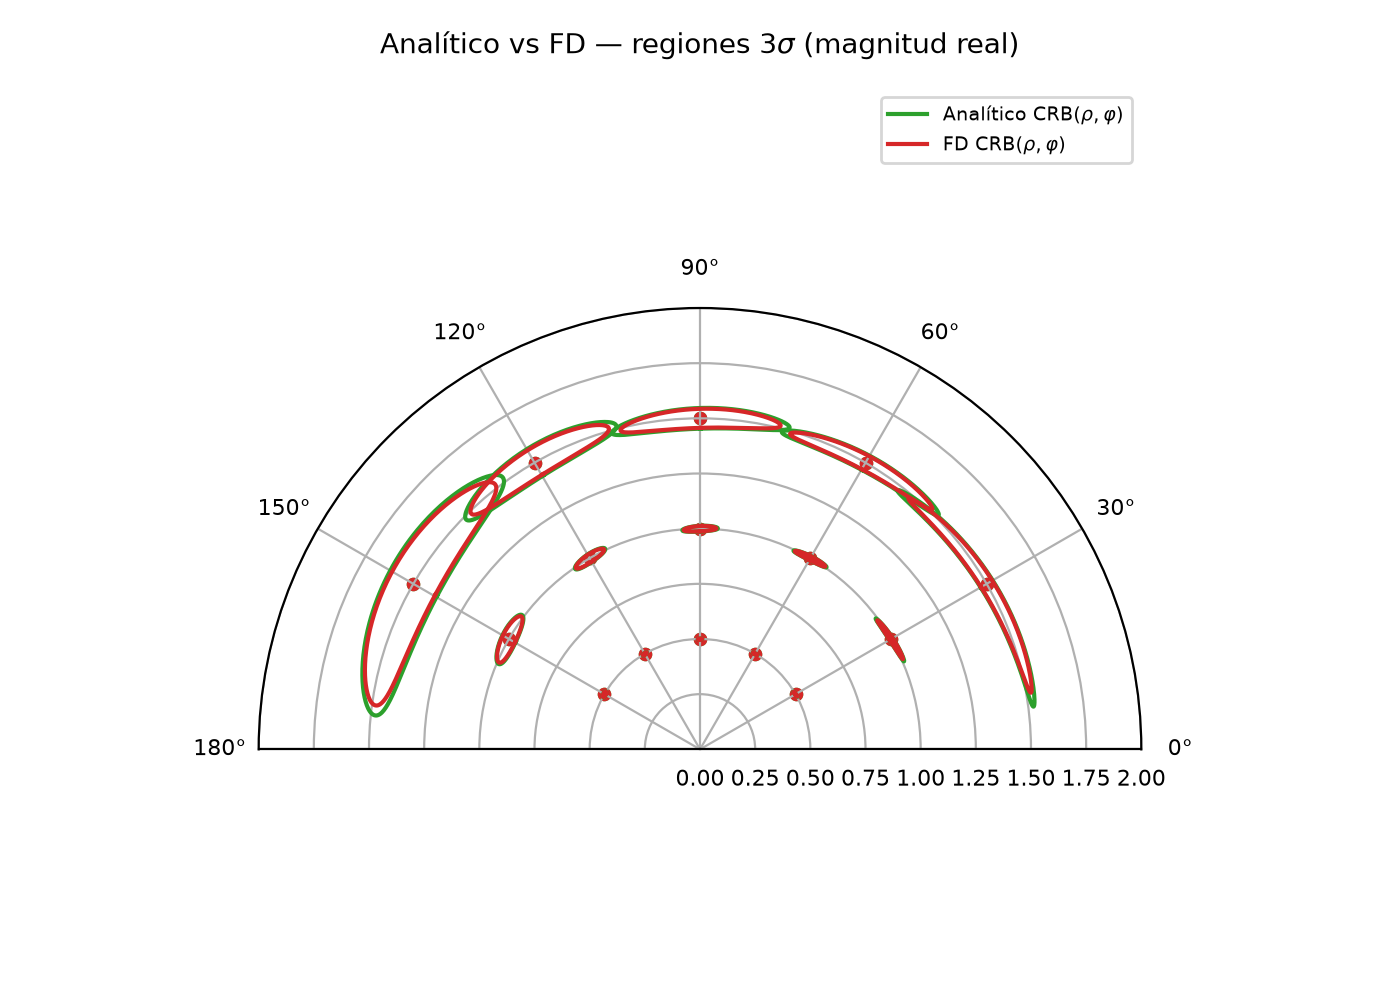
\includegraphics[width=\linewidth]{pr4_overlay.png}
  \caption{Rejilla completa.}
\end{subfigure}\hfill
\begin{subfigure}{0.48\textwidth}
  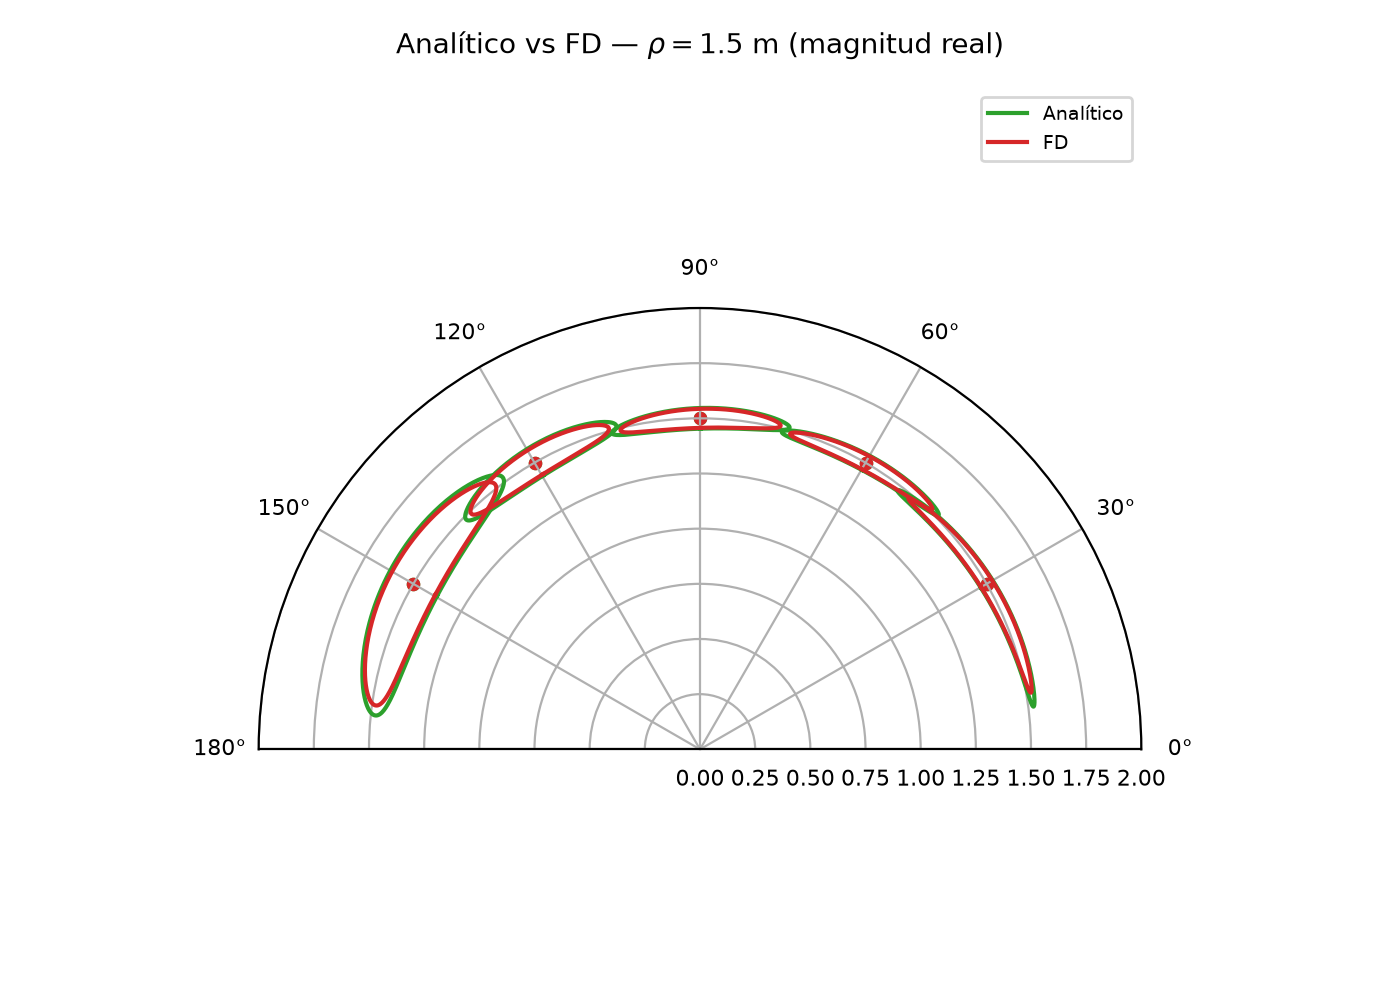
\includegraphics[width=\linewidth]{pr4_overlay_rho15.png}
  \caption{Detalle en $\rho=1.5\,$m, el caso más difícil.}
\end{subfigure}
\caption{PR\#4: superposición a magnitud real del CRB analítico (a)+(b)+(c)
sobre el FD. Las elipses caen una sobre otra sin ninguna normalización, en
ambos ejes.}
\label{fig:pr4}
\end{figure}

%=======================================================================
\section{Hallazgos de la revisión}
\label{sec:revision}

Todo el trabajo anterior se sometió a dos revisiones independientes: una
matemática (corrección de los \emph{forwards} analíticos y sus derivadas) y una
de código, figuras y documentación (ruta FD). Ambas trabajaron en modo lectura y
ejecutaron las validaciones para comprobar que los números citados se
reproducen.

\subsection{Lo que se verificó correcto}

\begin{itemize}[leftmargin=*]
  \item \textbf{Cero errores críticos.} Ninguna de las dos revisiones encontró
        errores matemáticos o de implementación que invaliden los resultados
        publicados. No hay errores de signo, de dirección de normales ni de
        constantes en ninguna rama.
  \item \textbf{Las derivadas simbólicas son correctas} en las tres ramas
        analíticas: jacobiano \code{sympy} frente a diferencia central del
        \emph{mismo} \emph{forward} suave da error máximo $5.0\cdot10^{-10}$
        (PR\#2), $9.7\cdot10^{-10}$ (PR\#3) y $5.5\cdot10^{-9}$ (PR\#4), todos
        muy por debajo del umbral de $10^{-6}$.
  \item \textbf{Los números publicados se reproducen exactamente}: tablas de
        validación, CRB de referencia, $\sigma$ de la rejilla y aspecto medio,
        en las tres ramas.
  \item \textbf{La ruta FD está correctamente implementada}: la diferencia
        central y la extrapolación de Richardson $(4D(\delta/2)-D(\delta))/3$
        son correctas; $\matr I = \matr J^\top\operatorname{diag}(1/g)\matr J$
        con piso $\varepsilon$ es correcta (y con fondo $0.1$ el piso nunca
        actúa); la elipse $3\sigma$ por descomposición espectral es la frontera
        correcta de $\{\vect\delta^\top\matr\Sigma^{-1}\vect\delta\le k^2\}$; y
        la matriz $A=\begin{psmallmatrix}\cos\varphi & -\rho\sin\varphi\\
        \sin\varphi & \rho\cos\varphi\end{psmallmatrix}$ \emph{es} el jacobiano
        de $(x,y)=(\rho\cos\varphi,\rho\sin\varphi)$, bien aplicada como
        $\matr\Sigma_{xy}=A\matr\Sigma A^\top$.
  \item \textbf{El \emph{placement} simbólico de PR\#4 replica exactamente} la
        celda 8 del \emph{notebook} (matrices de rotación verificadas contra
        \code{trimesh.rotation\_matrix}), con energía total coincidente al
        $0.03\%$.
\end{itemize}

\subsection{Claims corregidos}

\begin{finding}[La convergencia $128\to512$ triángulos no era $<0.5\%$]
\label{find:convergencia}
La documentación afirmaba que \enquote{los cambios de $128$ a $512$ y a $2048$
triángulos son $<0.5\%$}. Medido en $(\rho=1,\varphi=90^\circ)$ con la
configuración final: $128$ triángulos dan $\sigma_\rho=0.004248$ y $512$ dan
$0.004541$, es decir \textbf{$+6.9\%$}; el paso $512\to2048$ sí es $+0.37\%$.
En $\sigma_\varphi$: $+0.7\%$ y $+0.12\%$. La distinción correcta, que es la
que quedó documentada, es que la \textbf{energía} converge a $\approx128$
triángulos ($\approx0.1\%$, medido $0.137\%$, hasta $2048$), pero las
\textbf{$\sigma$ del CRB} ---que dependen de derivadas--- necesitan $\approx512$.
La configuración publicada ($512$) sí está razonablemente convergida, así que
los resultados se sostienen; era la justificación escrita la que estaba mal.
\end{finding}

\begin{finding}[Una \emph{caption} autogenerada contradecía su propia tabla]
\label{find:caption}
La función que escribía la tabla LaTeX de PR\#4 tenía la \emph{caption} con el
rango \enquote{$\sigma_\rho$ anal./FD $\approx0.9$--$1.05$} \textbf{escrito a mano},
mientras que las razones de la tabla adjunta son $1.08$--$1.10$ (todas $>1$), y
el propio abstract decía \enquote{$\approx10\%$}. Quedó corregido calculando el rango
mínimo--máximo a partir de los datos, con lo que ahora imprime $1.08$--$1.10$;
las filas de la tabla se verificaron byte-idénticas antes y después.
\end{finding}

\begin{finding}[\enquote{Converge hacia el FD} era incorrecto en PR\#3 y PR\#4]
Ya recogido como hallazgo~\ref{find:no-converge} para PR\#3. En PR\#4 la frase
\enquote{en el límite duro las Fisher coinciden} choca con la propia teoría del
documento (la proposición de inconsistencia de la FD: en el límite la derivada
diverge y la Fisher dura no existe clásicamente). Como heurística
---\enquote{ambas rutas ven la misma física}--- vale; como enunciado de convergencia, el
mismo documento lo refuta.
\end{finding}

\begin{finding}[El paso FD $\delta_\rho=0.01\,$m frente a la cuantización del
\emph{bin}]
\label{find:paso-fd}
Un \emph{bin} temporal vale $c\,\Delta t = 299792458\times3.9\cdot10^{-10}
\approx 0.1169\,$m de camino (ida y vuelta), es decir $\approx0.058\,$m en
$\rho$. Con $\delta_\rho=0.01\,$m, la diferencia central abarca $0.04\,$m de
camino, un \textbf{$34\%$ de un \emph{bin}}: para un triángulo aislado, la
mayoría de las evaluaciones $\pm\delta$ caen en el mismo \emph{bin} (meseta,
derivada temporal cero) y las que cruzan aportan saltos de masa $\propto
1/(2\delta_\rho)$. Lo que rescata a la ruta FD es la \textbf{densificación} de
la malla, que reparte las distancias por triángulo y auto-promedia el jacobiano
agregado. El estimador es razonable pero ruidoso y dependiente de $\delta$ ---lo
cual es coherente con que el modelo suave de PR\#4, con
$\tau=\Delta t/\sqrt{12}$, coincida con el FD dentro de un $10\%$.
Corolario práctico: \code{finite\_difference\_jacobian\_polar\_richardson} es
matemáticamente inapropiado sobre un \emph{forward} escalonado (la
extrapolación de Richardson supone una expansión del error en potencias de
$\delta$, que cerca de un salto no existe); no se usa en ningún \emph{script}
---siempre \code{central}---, pero conviene saberlo. Los otros pasos,
$\delta_\varphi=0.5^\circ$ y $\delta_h=0.01\,$m, sí son razonables.
\end{finding}

\begin{finding}[Fragilidad de las cachés]
\label{find:cache}
Dos problemas, ambos corregidos. Primero, la caché analítica
\code{crb\_grid\_results\_analytic.pkl} se reutilizaba a ciegas si contenía las
claves esperadas, y las \emph{tres} ramas analíticas usaban el \emph{mismo}
nombre de archivo para \emph{tres} modelos distintos: correr un \emph{script}
en un \emph{checkout} con la caché de otra variante habría producido figuras y
tablas obsoletas en silencio. Se resolvió estampando en el \emph{pickle} una
huella de configuración (\code{config\_key}) y recomputando con un aviso
explícito si no coincide. Segundo, la caché FD se resolvía por ruta absoluta
\code{/workspace/plots/crb\_grid\_results.pkl}, y en PR\#4 además en tiempo de
importación, lo que solo funciona en esa máquina con ese \emph{layout}.
\end{finding}

\subsection{Hallazgos menores}

\begin{itemize}[leftmargin=*]
  \item El \emph{docstring} de PR\#2 afirmaba \enquote{re-expresa la MISMA intensidad
        por píxel} que el simulador, lo cual no es cierto (faceta puntual en
        $z=h$, ganancia constante, rejilla propia). Se reescribió declarando
        explícitamente que es la variante base cualitativa, con una sección de
        salvedades honestas.
  \item La afirmación \enquote{$\kappa=60$ da una penumbra de $1.7\,$cm, comparable al
        tamaño de píxel} era falsa en ambos sentidos: el píxel de la rejilla
        propia de PR\#2 mide $6.25\,$cm y el del simulador $0.39\,$cm.
        Corregida a \enquote{valor genérico intermedio, no atado a ninguno}.
  \item Imprecisiones numéricas en la guía intuitiva: \enquote{PR\#3: $\sigma_\rho
        \approx0.5$--$0.7\times$ FD} cuando el rango real es $0.50$--$0.85$; y
        \enquote{razón $1.00$--$1.12$} para PR\#4 cuando el rango real es
        $1.08$--$1.10$ en $\sigma_\rho$ y $1.06$--$1.12$ en $\sigma_\varphi$.
        Corregidas.
  \item \code{\_pick\_zmin\_ref} usaba \emph{pitch}, \emph{roll} y escala
        codificados a mano en lugar de leerlos de la configuración; con los
        valores por defecto coincide, pero cambiar la configuración habría
        elegido el vértice de referencia equivocado sin aviso.
  \item El aspecto y la inclinación se miden en el plano de unidades mixtas
        $(\rho\,[\text{m}], \varphi\,[\text{rad}])$, de modo que los valores
        \enquote{aspecto $\approx8$} no son invariantes geométricos. Es una convención
        válida porque se aplica idéntica a ambos métodos, pero no debe leerse
        como una propiedad absoluta.
\end{itemize}

Tras aplicar las correcciones, se verificó que la rejilla publicada de PR\#4
quedó \textbf{bit-idéntica} (diferencia relativa máxima $0.00$) en cinco poses
de control, y que los PNG se regeneraron byte-idénticos.

%=======================================================================
\section{Estado final y decisiones}
\label{sec:final}

\begin{decision}[El simulador pasa a ser la implementación vectorizada en
PyTorch]
\label{dec:simulador}
El simulador de transientes se reemplaza por \code{simulator.py}, una
implementación en PyTorch que procesa \textbf{bloques de triángulos contra
todos los píxeles del SPAD a la vez} (parámetro
\code{triangle\_chunk\_size}, por defecto $256$), en lugar de enviar los
triángulos uno por uno. Detecta CUDA y cae a CPU si no está disponible. Además
de la simulación, genera conjuntos de datos completos en HDF5 (una carpeta por
escena con \code{transient.hdf5}, \code{scene.obj} y \code{meta.json}), con
muestreo aleatorio validado de posiciones de objeto e interfaz de línea de
comandos.

Se adoptó \textbf{tal cual}, sin cambios de diseño; la única modificación es
que \code{DEFAULT\_OBJECT\_FOLDER} apunta a la carpeta \code{objects/} real de
este repositorio en lugar de \code{obs/}. La función \code{simulation(...)}
devuelve \textbf{dos} valores, \code{(y\_meas\_vec\_noisy, params)}, tras
aplicar la reorientación \code{np.roll(..., shift=1, axis=1)}.
\end{decision}

\begin{decision}[La grilla de referencia baja de $64\times64$ a $32\times32$]
\label{dec:grilla}
El \emph{baseline} pasa a \code{cam\_pixel\_dim=32}. El resto de los parámetros
se mantiene coherente con lo que usaba el repositorio: FOV de cámara $0.25$,
$\Delta t = 3.9\cdot10^{-10}\,$s, $I_{\text{láser}}=1000$, paredes ocultas, sin
ruido, faceta \code{facet.obj} con $w=0.5\,$m, tasa de fondo $b=0.1$, y pasos de
diferencias finitas $(\delta_\rho,\delta_\varphi)=(0.01\,\text{m},0.5^\circ)$.
Reducir la grilla a la mitad en cada eje deja $1024$ píxeles en lugar de
$4096$, y el CRB empeora en consecuencia por un factor $\approx2$ en $\sigma$
(la información de Fisher es aditiva sobre píxeles, luego $\sigma$ escala como
la raíz del número de píxeles).
\end{decision}

\begin{decision}[El CRB de producción es el de FD con $\vect\psi=(\rho,\varphi)$
y Fisher $2\times2$; $\sigma_h$ deja de existir]
\label{dec:2param}
Esta es la consecuencia de modelado más importante de la
decisión~\ref{dec:simulador}, y conviene enunciarla sin rodeos.

El simulador nuevo escala la malla del objeto con
%
\begin{equation}
\text{escala} = \min\!\left(\frac{w}{\text{extents}_x},\;
                            \frac{1.1}{\text{extents}_z}\right),
\end{equation}
%
y \textbf{no lee en ningún momento una clave \code{h}}: la altura del objeto no
es una entrada controlable, sino un resultado de la geometría de la malla y de
la anchura $w$. Por tanto \textbf{no existe la derivada $\partial g/\partial h$
y no puede definirse $\sigma_h$}. El vector de parámetros del CRB queda
reducido a $\vect\psi=(\rho,\varphi)$, la matriz de información de Fisher es
$2\times2$, y hay que llamar al CRB con \code{estimate\_height=False}.

Consecuencias concretas: desaparece toda la familia de resultados
\enquote{$\text{CRB}(\rho,\varphi,h)$ / Fisher $3\times3$} que aparecía en PR\#1
(figura~\ref{fig:pr1}b) y la comparación $2$ frente a $3$ parámetros. Si en el
futuro se quiere recuperar $\sigma_h$, hay que \emph{añadir} al simulador una
entrada de altura explícita ---lo que sería un cambio de diseño del código
aportado, no una adaptación---; mientras eso no ocurra, la altura es un parámetro
de nuisance fijado por la geometría, no estimable.
\end{decision}

\subsection{Cómo se conectan el CRB y el simulador nuevo}

Hay una incompatibilidad de interfaz que merece quedar registrada. La función
%
\begin{center}
\code{crb\_polar\_functions.simulate\_facet\_signal\_expected}
\end{center}
%
desempaqueta \textbf{tres} valores del \emph{callable} de simulación,
%
\begin{center}
\code{\_, y\_signal, params = simulation\_fn(**kwargs)},
\end{center}
%
herencia del simulador del \emph{notebook}, que devolvía
\code{(ruidoso, limpio, params)}. El simulador nuevo devuelve \textbf{dos}.

Se adaptó \textbf{el lado del CRB}, no el simulador. Un adaptador delgado,
%
\begin{center}
\code{crb\_fd\_baseline.simulation\_fn\_for\_crb},
\end{center}
%
llama a \code{simulator.simulation} y re-emite su par $(y,\text{params})$ como
la terna $(y, y, \text{params})$ que el CRB espera.

La adaptación es legítima y no pierde información porque el CRB siempre invoca
el \emph{forward} con \code{force\_no\_noise=True}, que fija
\code{add\_noise=False}; en ese caso el único transiente devuelto \emph{es} la
señal esperada sin ruido, así que puede ocupar legítimamente ambas ranuras. El
adaptador falla de forma explícita si se le pasa \code{add\_noise=True}.
Con este diseño, \code{crb\_polar\_functions.py} \textbf{no se modificó en
absoluto}.

Dos notas menores de compatibilidad: el diccionario de posición de objeto que
construye el CRB incluye claves \code{h} y \code{yaw} que el simulador nuevo
simplemente ignora (no fallan); y el \emph{baseline} usa \code{torch.float64}
porque las diferencias centrales con pasos de $1\,$cm y $0.5^\circ$ producen
diferencias de intensidad por \emph{bin} en las que el redondeo de
\code{float32} sería una fracción apreciable.

\subsection{Resultados del CRB por FD con el \emph{baseline} $32\times32$}

La tabla~\ref{tab:baseline} es el resultado de referencia del repositorio a
partir de ahora. Se obtuvo ejecutando \code{compute\_crb\_fd\_baseline.py}
completo: $15$ poses, $5$ evaluaciones del \emph{forward} por pose (una central
y cuatro perturbadas), en $77.2\,$s totales, es decir $5.15\,$s por pose en CPU
con \code{float64}. Cada evaluación produce un transiente de
$32\times32\times95$ \emph{bins}, o $97\,280$ observaciones de Poisson.

\begin{table}[htbp]
\centering
\caption{\emph{Baseline} final: CRB$(\rho,\varphi)$ por diferencias finitas
sobre el simulador PyTorch, grilla $32\times32$, Fisher $2\times2$. La columna
$\rho\,\sigma_\varphi$ es el error tangencial y $r_{\rho\varphi}$ la
correlación entre ambos parámetros. No hay columna $\sigma_h$: no está definida
(decisión~\ref{dec:2param}).}
\label{tab:baseline}
\begin{tabular}{@{}rr rrrr@{}}
\toprule
$\rho$ [m] & $\varphi$ [$^\circ$] & $\sigma_\rho$ [m]
& $\sigma_\varphi$ [$^\circ$] & $\rho\,\sigma_\varphi$ [m]
& $r_{\rho\varphi}$ \\
\midrule
0.50 & 30 & 0.00136 & 1.003 & 0.008757 & -0.731 \\
0.50 & 60 & 0.001352 & 0.8721 & 0.00761 & -0.583 \\
0.50 & 90 & 0.001556 & 0.7535 & 0.006576 & -0.435 \\
0.50 & 120 & 0.002223 & 0.8106 & 0.007074 & -0.402 \\
0.50 & 150 & 0.003695 & 1.087 & 0.009487 & -0.403 \\
\midrule
1.00 & 30 & 0.006852 & 3.717 & 0.06488 & -0.564 \\
1.00 & 60 & 0.007162 & 2.714 & 0.04736 & -0.379 \\
1.00 & 90 & 0.008795 & 2.574 & 0.04493 & -0.283 \\
1.00 & 120 & 0.01318 & 2.67 & 0.04661 & -0.250 \\
1.00 & 150 & 0.02271 & 4.159 & 0.07259 & -0.256 \\
\midrule
1.50 & 30 & 0.02566 & 10.77 & 0.282 & -0.452 \\
1.50 & 60 & 0.02775 & 7.32 & 0.1916 & -0.280 \\
1.50 & 90 & 0.03482 & 7.29 & 0.1908 & -0.209 \\
1.50 & 120 & 0.05176 & 7.381 & 0.1932 & -0.191 \\
1.50 & 150 & 0.09031 & 11.69 & 0.3059 & -0.184 \\
\bottomrule
\end{tabular}
\end{table}

\begin{figure}[htbp]
\centering
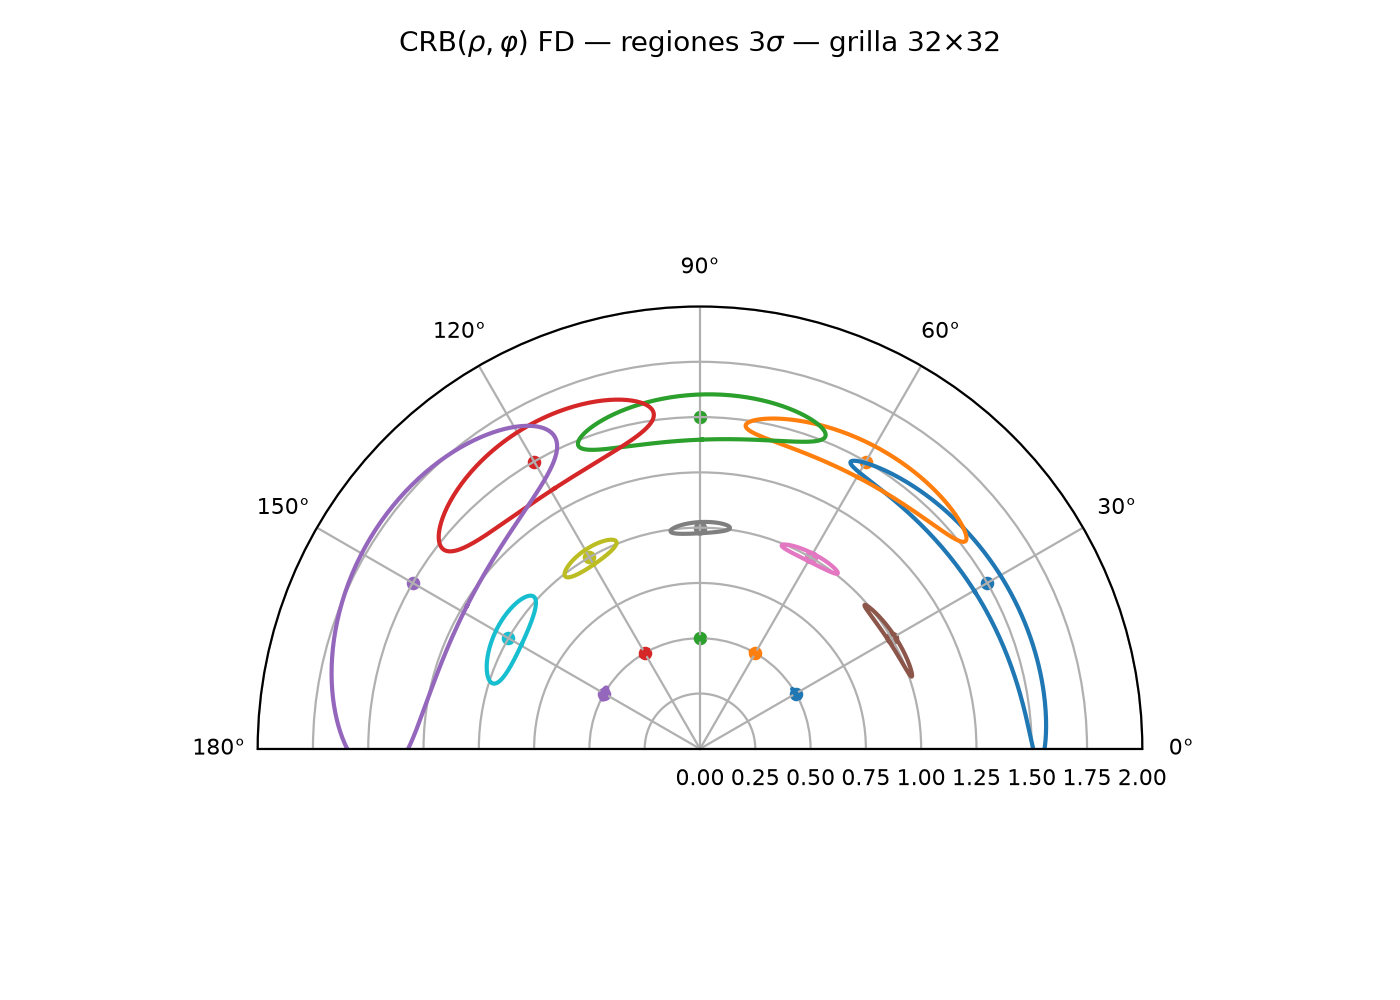
\includegraphics[width=0.72\textwidth]{fd_baseline_32.png}
\caption{Regiones $3\sigma$ del CRB$(\rho,\varphi)$ por diferencias finitas
sobre el simulador PyTorch con la grilla $32\times32$. Es la figura de
referencia del repositorio; se regenera con
\code{python3 compute\_crb\_fd\_baseline.py}.}
\label{fig:baseline}
\end{figure}

\paragraph{Lectura de los resultados.}
Las tres tendencias son las esperadas y coinciden cualitativamente con todo el
estudio anterior:
%
\begin{itemize}[leftmargin=*]
  \item \textbf{La precisión se degrada rápido con la distancia.} De $\rho=0.5$
        a $\rho=1.5\,$m, $\sigma_\rho$ crece más de un factor $20$
        ($1.4\,$mm $\to 2.6$--$9.0\,$cm). El transiente de dos rebotes decae
        como $1/(d_1^2 d_2^2)$, así que la señal se desvanece muy rápido.
  \item \textbf{El ángulo es más incierto en los extremos.} Para cada $\rho$,
        $\sigma_\varphi$ es mínima cerca de $\varphi=90^\circ$ (frente al
        sensor) y máxima en $\varphi=30^\circ$ y $150^\circ$. En
        $\varphi=150^\circ$ el objeto está más ocluido por la arista y aporta
        menos información azimutal.
  \item \textbf{$\rho$ y $\varphi$ están anticorrelacionados}
        ($r_{\rho\varphi}$ entre $-0.18$ y $-0.73$), lo que es la razón por la
        que las burbujas de la figura~\ref{fig:baseline} aparecen inclinadas y
        no alineadas con los ejes: un error de rango puede compensarse
        parcialmente con un error de ángulo manteniendo un tiempo de vuelo
        similar.
  \item \textbf{El error tangencial $\rho\,\sigma_\varphi$ domina el error
        radial} en todas las poses, por un factor de $4$ a $6$. La cámara de
        esquina localiza el rango mucho mejor que el azimut, que es
        exactamente la anisotropía que las elipses muy alargadas
        (aspecto $\approx8$) venían mostrando en todo el estudio.
\end{itemize}

Comparando con la referencia FD anterior a $64\times64$ (tabla~\ref{tab:pr4},
columnas FD), la degradación por bajar a $32\times32$ es de un factor
$\approx1.9$--$2.4$ en $\sigma_\rho$ y $\approx1.6$--$1.9$ en
$\sigma_\varphi$, consistente con la aditividad de la información de Fisher
sobre los píxeles.

\subsection{Qué quedó en el repositorio y qué se retiró}

La rama consolidada conserva únicamente la documentación, el simulador nuevo, el
\emph{pipeline} del CRB por diferencias finitas y sus utilidades y objetos. Todo
lo retirado se comprobó previamente sin referencias (con \code{grep}), y después
de retirarlo se volvió a ejecutar el \emph{pipeline} completo: el
\emph{smoke test} del simulador y un recálculo con \code{--force} de las $15$
poses reproducen sus números anteriores, y
\code{plots/crb\_fd\_baseline\_32.png} se regenera byte-idéntico.

\paragraph{Retirado.}
\begin{itemize}[leftmargin=*]
  \item \code{pyerti.py} --- el simulador antiguo en CPU. Superado por
        \code{simulator.py}; nadie lo importaba y su carpeta de objetos apuntaba
        a un directorio \code{NLOS-Simulator/} inexistente.
  \item \code{regenerate\_crb\_standard\_regions.py} --- obtenía la función de
        simulación ejecutando (\code{exec}) las celdas $1,3,5,7,8$ del
        \emph{notebook}. Superado por \code{compute\_crb\_fd\_baseline.py}.
        Calculaba además el CRB de tres parámetros, que el simulador nuevo no
        puede sostener (decisión~\ref{dec:2param}).
  \item \code{simulation\_polar\_clean.ipynb}, \code{simulation.ipynb} y
        \code{validation.ipynb} --- unos $9\,$MB de \emph{notebooks}. El primero
        solo lo referenciaba el \emph{script} anterior; los otros dos, nada. Su
        contenido queda documentado en este reporte.
  \item \code{plots/crb\_standard\_regions.png} y
        \code{plots/crb\_standard\_regions\_fixed\_h.png} --- salidas del
        \emph{script} retirado, calculadas sobre el simulador antiguo a
        $64\times64$. Las versiones mejoradas de esos mismos resultados se
        conservan en \code{docs/figs\_consolidado/} y están incrustadas en la
        figura~\ref{fig:pr1}.
\end{itemize}

\paragraph{Conservado a propósito, aunque el \emph{pipeline} no lo use.}
\begin{itemize}[leftmargin=*]
  \item \code{sr\_crb.py} --- un barrido de resolución de cámara, directamente
        pertinente a la elección de la grilla de $32\times32$. Está
        \textbf{roto} en este momento: \code{utils/crb\_utils.py} es un archivo
        de $0$ bytes, de modo que \code{sr\_crb.py} ni se importa. Se conserva
        porque documenta la interfaz que se pretendía
        (\code{SimulationConfig}, \code{run\_sweep},
        \code{plot\_range\_angle\_sweep}) y porque el barrido sería útil para
        justificar cuantitativamente la grilla.
  \item \code{objects/validation.ipynb} --- inerte, porque
        \code{get\_obj\_files} solo busca \code{*.obj}, y situado en una ruta
        protegida.
  \item \code{utils/NLOS\_simulator.py} y \code{utils/crb\_fix.py} --- código de
        simulación anterior, bajo \code{utils/}, que se conserva íntegro.
\end{itemize}

%=======================================================================
\section{Catálogo de figuras}
\label{sec:catalogo}

Todas las figuras de este documento están en \code{docs/figs\_consolidado/} y
provienen de las ramas indicadas. Se conservan aquí porque las ramas se
retiran.

\small
\begin{longtable}{@{}p{5.4cm}p{1.6cm}p{8.1cm}@{}}
\toprule
Archivo & Origen & Qué muestra \\
\midrule
\endfirsthead
\toprule
Archivo & Origen & Qué muestra \\
\midrule
\endhead
\code{fd\_baseline\_32.png} & actual &
  \textbf{Figura de referencia actual}: burbujas $3\sigma$ del
  CRB$(\rho,\varphi)$ por FD sobre el simulador PyTorch a $32\times32$
  (figura~\ref{fig:baseline}). \\
\addlinespace
\code{pr1\_fd\_fixed\_h.png} & PR\#1 &
  CRB$(\rho,\varphi)$ por FD, Fisher $2\times2$, simulador antiguo a
  $64\times64$. \\
\code{pr1\_fd\_with\_h.png} & PR\#1 &
  CRB$(\rho,\varphi,h)$ por FD, Fisher $3\times3$, proyectado en
  $(\rho,\varphi)$. Ya no reproducible: el simulador nuevo no tiene entrada de
  altura (decisión~\ref{dec:2param}). \\
\code{pr1\_fd\_compare\_2\_vs\_3.png} & PR\#1 &
  Comparación lado a lado y superpuesta de $2$ frente a $3$ parámetros.
  También histórica, por la misma razón. \\
\addlinespace
\code{pr2\_analytic\_fixed\_h.png} & PR\#2 &
  Burbujas del CRB analítico base, en su propia escala (no comparable en
  magnitud). \\
\code{pr2\_shapenorm.png} & PR\#2 &
  Superposición normalizada en forma, analítico (verde) frente a FD (rojo):
  la única comparación honesta en esa rama. \\
\addlinespace
\code{smoothing\_binning.png} & PR\#4 &
  El reemplazo $\lceil\cdot\rceil\to\erf$, con la conservación de masa del
  \emph{kernel}. \\
\code{smoothing\_occlusion.png} & PR\#4 &
  El reemplazo escalón $\to$ sigmoide, con la penumbra de un píxel
  ($\kappa=256$). \\
\code{smoothing\_foreshortening.png} & PR\#4 &
  El reemplazo $\max(0,\cdot)\to$ \emph{softplus} en los cosenos. \\
\addlinespace
\code{pr3\_overlay.png} & PR\#3 &
  Superposición a magnitud real (a)+(b) sobre FD: escalas correctas, elipses
  sistemáticamente pequeñas por el sesgo de cuadratura puntual
  (hallazgo~\ref{find:cuadratura}). \\
\addlinespace
\code{pr4\_overlay.png} & PR\#4 &
  Superposición a magnitud real (a)+(b)+(c) sobre FD: coincidencia en ambos
  ejes dentro del $10\%$. \\
\code{pr4\_overlay\_rho15.png} & PR\#4 &
  El mismo detalle restringido a $\rho=1.5\,$m, el caso más difícil. \\
\bottomrule
\end{longtable}

\subsection{Documentos originales y dónde quedan sus contenidos}

\begin{itemize}[leftmargin=*]
  \item \code{docs/sustento\_teorico\_crb.tex} (en \code{main}): sustento
        teórico del CRB de la implementación. \textbf{Se conserva en el
        repositorio.}
  \item \code{docs/analytic\_forward\_crb.tex} (PR\#2, PR\#3, PR\#4, una
        versión por rama): la construcción paso a paso del \emph{forward}
        diferenciable, la derivada analítica, y la justificación matemática con
        los teoremas de la función implícita, Rademacher, convergencia
        dominada, Leibniz y \emph{mollifiers}. Sus contenidos se resumen en la
        sección~\ref{sec:crb} y sus resultados en la
        sección~\ref{sec:cronologia}.
  \item \code{docs/guia\_intuitiva.tex} (PR\#4): guía en lenguaje llano, con el
        mapa de ramas y el catálogo de \emph{plots}. Su material se refleja en
        las secciones~\ref{sec:crb} y~\ref{sec:catalogo}.
  \item \code{docs/analytic\_vs\_fd\_comparison.txt} (PR\#2, PR\#3, PR\#4): las
        tablas numéricas comparativas. Reproducidas íntegras en las
        tablas~\ref{tab:pr2}, \ref{tab:pr3} y~\ref{tab:pr4}.
\end{itemize}

%=======================================================================
\section{Cómo reproducir el estado final}
\label{sec:reproducir}

\begin{enumerate}[leftmargin=*]
  \item Dependencias (la versión de CPU de \code{torch} basta: el código
        detecta CUDA y cae a CPU si no la hay):
        \begin{center}\code{pip install -r requirements.txt}\end{center}
  \item Simulación suelta o generación de un conjunto de datos en HDF5:
        \begin{center}
        \code{python3 simulator.py --num-scenes 4 --cam-pixel-dim 32 --device auto}
        \end{center}
  \item CRB de referencia:
        \begin{center}\code{python3 compute\_crb\_fd\_baseline.py}\end{center}
        Cachea en \code{plots/crb\_fd\_baseline\_32.pkl} (ignorado por git) y
        escribe \code{plots/crb\_fd\_baseline\_32.png}. Con \code{--force}
        recomputa ignorando la caché, y con \code{--cam-pixel-dim N} evalúa
        otra grilla.
\end{enumerate}

\end{document}
